\chapter{Appendix}
    \section{Table of Frequently Used Expressions \label{frequentExpressions}}
    
    \begin{center}
    \begin{tabular}{|c|c|c|c|}
     \hline
    \multicolumn{4}{|c|}{\textbf{List of Frequent Expressions in Stack Overflow and Github data}} \\
     \hline
    web\_services & jupyter\_notebook & machine\_learning & visual\_studio  \\
    objective\_c & unit\_testing & deep\_learning & artificial\_intelligence  \\
    vim\_script & data\_visualization & data\_science & software\_engineering   \\
    front\_end & android\_sdk & google\_analytics & android\_development  \\
    mac\_os & web\_application & data\_analysis & functional\_programming  \\
    web\_design & restful\_api & image\_processing & web\_development  \\
    emacs\_lisp & software\_design & data\_structures & app\_development \\
     \hline
    \end{tabular}
    \end{center}
    
    
    \section{Expertise Study Details \label{surveyAppendix}}
        \subsection{Sample Expertise Study}
            \begin{figure}
                \centerline{
                  \subfigure[Section I]{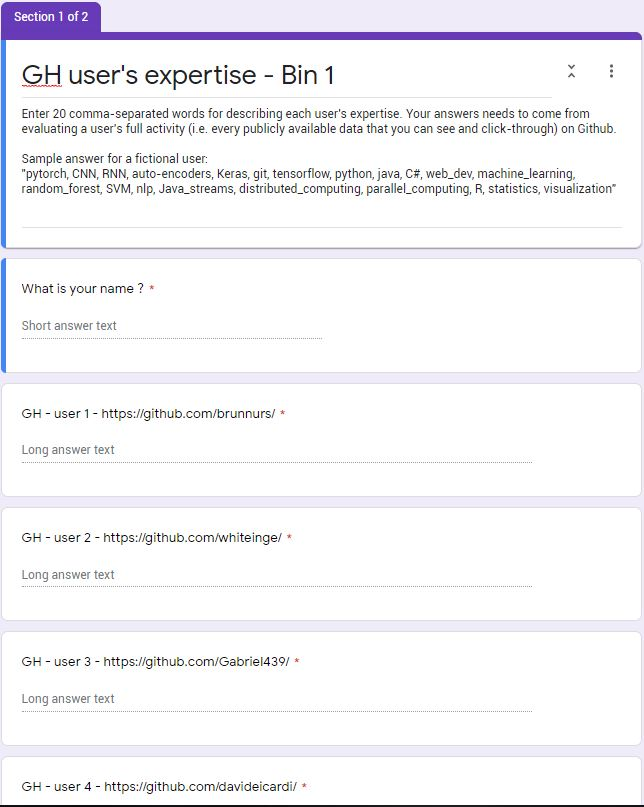
\includegraphics[width=3in]{figures/survey1.JPG}}\hfil
                  \subfigure[Section II]{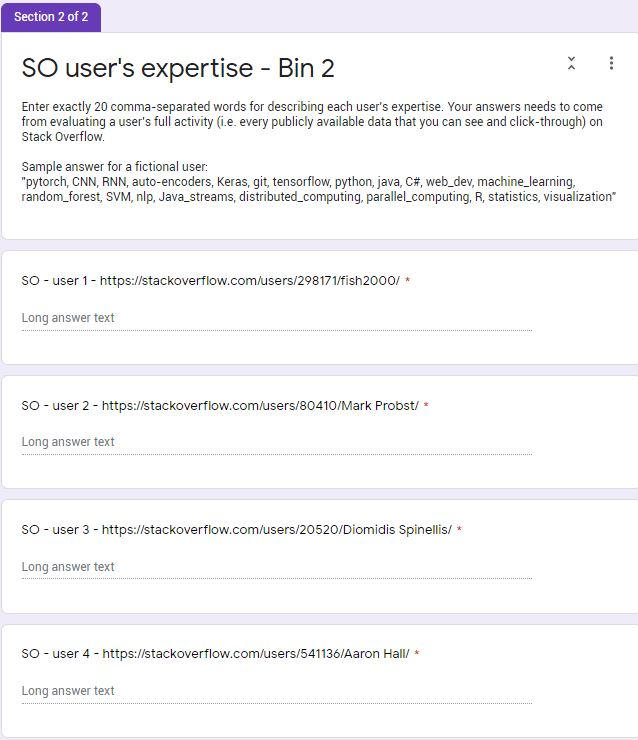
\includegraphics[width=3in]{figures/survey2.JPG}} }
                \caption{Sample Google Form Expertise Study} \label{fig:sampleSurvey}
            \end{figure}
        
        \subsection{Stack Overflow User Profile URLs in Expertise Study}
        
            \begin{center}
            \begin{longtable}{|p{1.5cm}|p{12.5cm}|}
            \caption{List of Stack Overflow User Profile URLs in Study} \label{survey_SO_userURLS} \\
             \hline
            \textbf{Sample} & \textbf{Stack Overflow User Profile URL} \\
             \hline
            1 & https://stackoverflow.com/users/1081551/u\_b/  \\
            2 & https://stackoverflow.com/users/127816/whiteinge/  \\
            3 & https://stackoverflow.com/users/1026598/Gabriel Gonzalez/  \\
            4 & https://stackoverflow.com/users/209727/Davide Icardi/  \\
            5 & https://stackoverflow.com/users/562883/Jonathan Stray/  \\
            6 & https://stackoverflow.com/users/369874/Paul Kehrer/  \\
            7 & https://stackoverflow.com/users/94559/smarx/  \\
            8 & https://stackoverflow.com/users/102441/Eric/  \\
            9 & https://stackoverflow.com/users/1270695/A5C1D2H2I1M1N2O1R2T1/  \\
            10 & https://stackoverflow.com/users/456809/Breedly/ \\
            11 & https://stackoverflow.com/users/298171/fish2000/ \\
            12 & https://stackoverflow.com/users/80410/Mark Probst/ \\
            13 & https://stackoverflow.com/users/20520/Diomidis Spinellis/ \\
            14 & https://stackoverflow.com/users/541136/Aaron Hall/ \\
            15 & https://stackoverflow.com/users/14955/Thilo/ \\
            16 & https://stackoverflow.com/users/272689/vimalloc/ \\
            17 & https://stackoverflow.com/users/1006669/Giovanni Lovato/ \\
            18 & https://stackoverflow.com/users/101152/Karel Bílek/ \\
            19 & https://stackoverflow.com/users/65311/devth/ \\
            20 & https://stackoverflow.com/users/529187/Xiao Peng - ZenUML.com/ \\
            21 & https://stackoverflow.com/users/470682/mkso/ \\
            22 & https://stackoverflow.com/users/763799/basgys/ \\
            23 & https://stackoverflow.com/users/446536/geon/ \\
            24 & https://stackoverflow.com/users/1162018/Daniel Iser/ \\
            25 & https://stackoverflow.com/users/257568/ArtemGr/ \\
            26 & https://stackoverflow.com/users/43839/Tom Swirly/ \\
            27 & https://stackoverflow.com/users/24998/Jack/ \\
            28 & https://stackoverflow.com/users/1190453/danbst/  \\
            29 & https://stackoverflow.com/users/870615/qwtel/  \\
            30 & https://stackoverflow.com/users/557368/rosenfeld/  \\
            31 & https://stackoverflow.com/users/33518/Tomas Petricek/  \\
            32 & https://stackoverflow.com/users/492393/Dmitrii Sorin/  \\
            33 & https://stackoverflow.com/users/177275/Yurik/ \\
            34 & https://stackoverflow.com/users/324790/Ivan Nikolaev/ \\
            35 & https://stackoverflow.com/users/554531/Keith Hughitt/ \\
            36 & https://stackoverflow.com/users/1074377/Kage/ \\
            37 & https://stackoverflow.com/users/20394/Mike Samuel/ \\
            38 & https://stackoverflow.com/users/94148/aleung/ \\
            39 & https://stackoverflow.com/users/1051598/Roman  Elizarov/ \\
            40 & https://stackoverflow.com/users/736714/deitch/ \\
            41 & https://stackoverflow.com/users/239247/anatoly techtonik/ \\
            42 & https://stackoverflow.com/users/747768/Kirill Dmitrenko/ \\
            43 & https://stackoverflow.com/users/663505/pirxpilot/ \\
            44 & https://stackoverflow.com/users/227267/Matti Virkkunen/ \\
            45 & https://stackoverflow.com/users/1968/Konrad Rudolph/ \\
            46 & https://stackoverflow.com/users/511200/danneu/ \\
            47 & https://stackoverflow.com/users/161801/asmeurer/ \\
            48 & https://stackoverflow.com/users/613198/rsp/ \\
            49 & https://stackoverflow.com/users/1457000/Adam D. Ruppe/ \\
            50 & https://stackoverflow.com/users/1294964/Marko Lukša/ \\
            51 & https://stackoverflow.com/users/7122/David Arno/ \\
            52 & https://stackoverflow.com/users/214488/memo/ \\
            53 & https://stackoverflow.com/users/246616/mVChr/ \\
            54 & https://stackoverflow.com/users/180783/astrofrog/ \\
            55 & https://stackoverflow.com/users/159695/Galaxy/ \\
            56 & https://stackoverflow.com/users/512596/Joey/ \\
            57 & https://stackoverflow.com/users/248296/warvariuc/ \\
            58 & https://stackoverflow.com/users/173314/wjt/ \\
            59 & https://stackoverflow.com/users/1305344/Jacek Laskowski/ \\
            60 & https://stackoverflow.com/users/561698/Andrew/ \\
            61 & https://stackoverflow.com/users/875915/Rob Bednark/ \\
            62 & https://stackoverflow.com/users/135786/Ben Lesh/ \\
            63 & https://stackoverflow.com/users/11543/mjs/ \\
            64 & https://stackoverflow.com/users/1048571/Jon Douglas/ \\
            65 & https://stackoverflow.com/users/1463744/fagiani/ \\
            66 & https://stackoverflow.com/users/308174/Larry Cai/ \\
            67 & https://stackoverflow.com/users/267416/Islam Wazery/ \\
            68 & https://stackoverflow.com/users/3109/MatthieuGD/ \\
            69 & https://stackoverflow.com/users/297131/Evgenii/ \\
            70 & https://stackoverflow.com/users/1240763/Gary Russell/ \\
            71 & https://stackoverflow.com/users/11238/Randy Sugianto 'Yuku'/ \\
            72 & https://stackoverflow.com/users/477476/Cactus/ \\
            73 & https://stackoverflow.com/users/211327/Alan H./ \\
            74 & https://stackoverflow.com/users/146041/Aaron McDaid/ \\
            75 & https://stackoverflow.com/users/503899/kraenhansen/ \\
            76 & https://stackoverflow.com/users/81071/Koraktor/ \\
            77 & https://stackoverflow.com/users/632242/Leszek/ \\
            78 & https://stackoverflow.com/users/537554/ryenus/ \\
            79 & https://stackoverflow.com/users/242457/David Jones/ \\
            80 & https://stackoverflow.com/users/62600/Todd Menier/ \\
            81 & https://stackoverflow.com/users/136285/malat/ \\
            82 & https://stackoverflow.com/users/163197/danielkza/ \\
            83 & https://stackoverflow.com/users/744520/Jacques Kvam/ \\
            84 & https://stackoverflow.com/users/14405/Robin like the bird/ \\
            85 & https://stackoverflow.com/users/1282247/dodomorandi/ \\
            86 & https://stackoverflow.com/users/771848/alecxe/ \\
            87 & https://stackoverflow.com/users/397020/Adron/ \\
            88 & https://stackoverflow.com/users/1209004/johan/ \\
            89 & https://stackoverflow.com/users/435093/slhck/ \\
            90 & https://stackoverflow.com/users/408195/Diogo Melo/ \\
            91 & https://stackoverflow.com/users/432903/prayagupd/ \\
            92 & https://stackoverflow.com/users/341772/Max/ \\
            93 & https://stackoverflow.com/users/189599/Antonello/ \\
            94 & https://stackoverflow.com/users/501266/Keith Bennett/ \\
            95 & https://stackoverflow.com/users/208809/Gordon/ \\
            96 & https://stackoverflow.com/users/541949/ivoba/ \\
            97 & https://stackoverflow.com/users/241510/Ruudjah/ \\
            98 & https://stackoverflow.com/users/771838/rossta/ \\
            99 & https://stackoverflow.com/users/933228/petrelharp/ \\
            100 & https://stackoverflow.com/users/552182/Muaz Khan/ \\
            \hline
            \end{longtable}
            \end{center}
        
        \subsection{GitHub User Profile URLs in Expertise Study}
        
            \begin{center}
            \begin{longtable}{|p{2cm}|p{7cm}|}
            \caption{List of GitHub User Profile URLs in Study} \label{survey_GH_userURLS} \\
             \hline
            \textbf{Sample ID} & \textbf{GitHub User Profile URL} \\
             \hline
            1 & https://github.com/brunnurs/ \\
            2 & https://github.com/whiteinge/ \\
            3 & https://github.com/Gabriel439/ \\
            4 & https://github.com/davideicardi/ \\
            5 & https://github.com/jstray/ \\
            6 & https://github.com/reaperhulk/ \\
            7 & https://github.com/smarx/ \\
            8 & https://github.com/eric-wieser/ \\
            9 & https://github.com/mrdwab/ \\
            10 & https://github.com/Freyert/ \\
            11 & https://github.com/fish2000/ \\
            12 & https://github.com/schani/ \\
            13 & https://github.com/dspinellis/ \\
            14 & https://github.com/aaronchall/ \\
            15 & https://github.com/thiloplanz/ \\
            16 & https://github.com/vimalloc/ \\
            17 & https://github.com/heruan/ \\
            18 & https://github.com/runn1ng/ \\
            19 & https://github.com/devth/ \\
            20 & https://github.com/MrCoder/ \\
            21 & https://github.com/khanmurtuza/ \\
            22 & https://github.com/basgys/ \\
            23 & https://github.com/geon/ \\
            24 & https://github.com/danieliser/ \\
            25 & https://github.com/ArtemGr/ \\
            26 & https://github.com/rec/ \\
            27 & https://github.com/jacktasia/ \\
            28 & https://github.com/danbst/ \\
            29 & https://github.com/qwtel/ \\
            30 & https://github.com/rosenfeld/ \\
            31 & https://github.com/tpetricek/ \\
            32 & https://github.com/1999/ \\
            33 & https://github.com/nyurik/ \\
            34 & https://github.com/V0idExp/ \\
            35 & https://github.com/khughitt/ \\
            36 & https://github.com/kjjgibson/ \\
            37 & https://github.com/mikesamuel/ \\
            38 & https://github.com/aleung/ \\
            39 & https://github.com/elizarov/ \\
            40 & https://github.com/deitch/ \\
            41 & https://github.com/techtonik/ \\
            42 & https://github.com/dmikis/ \\
            43 & https://github.com/pirxpilot/ \\
            44 & https://github.com/mvirkkunen/ \\
            45 & https://github.com/klmr/ \\
            46 & https://github.com/danneu/ \\
            47 & https://github.com/asmeurer/ \\
            48 & https://github.com/rsp/ \\
            49 & https://github.com/adamdruppe/ \\
            50 & https://github.com/luksa/ \\
            51 & https://github.com/DavidArno/ \\
            52 & https://github.com/memo/ \\
            53 & https://github.com/mreinhardt/ \\
            54 & https://github.com/astrofrog/ \\
            55 & https://github.com/galaxy001/ \\
            56 & https://github.com/joeyh/ \\
            57 & https://github.com/warvariuc/ \\
            58 & https://github.com/wjt/ \\
            59 & https://github.com/jaceklaskowski/ \\
            60 & https://github.com/almartin82/ \\
            61 & https://github.com/RobBednark/ \\
            62 & https://github.com/blesh/ \\
            63 & https://github.com/ithinkihaveacat/ \\
            64 & https://github.com/JonDouglas/ \\
            65 & https://github.com/fagiani/ \\
            66 & https://github.com/larrycai/ \\
            67 & https://github.com/wazery/ \\
            68 & https://github.com/matthieugd/ \\
            69 & https://github.com/evgenyneu/ \\
            70 & https://github.com/garyrussell/ \\
            71 & https://github.com/yukuku/ \\
            72 & https://github.com/gergoerdi/ \\
            73 & https://github.com/alanhogan/ \\
            74 & https://github.com/aaronmcdaid/ \\
            75 & https://github.com/kraenhansen/ \\
            76 & https://github.com/koraktor/ \\
            77 & https://github.com/lpryszcz/ \\
            78 & https://github.com/ryenus/ \\
            79 & https://github.com/drj11/ \\
            80 & https://github.com/tmenier/ \\
            81 & https://github.com/malaterre/ \\
            82 & https://github.com/danielkza/ \\
            83 & https://github.com/jwkvam/ \\
            84 & https://github.com/RobinIsTheBird/ \\
            85 & https://github.com/dodomorandi/ \\
            86 & https://github.com/alecxe/ \\
            87 & https://github.com/Adron/ \\
            88 & https://github.com/bitsgalore/ \\
            89 & https://github.com/slhck/ \\
            90 & https://github.com/dmelo/ \\
            91 & https://github.com/prayagupd/ \\
            92 & https://github.com/nanodeath/ \\
            93 & https://github.com/tsutomi/ \\
            94 & https://github.com/keithrbennett/ \\
            95 & https://github.com/gooh/ \\
            96 & https://github.com/ivoba/ \\
            97 & https://github.com/generateui/ \\
            98 & https://github.com/rossta/ \\
            99 & https://github.com/petrelharp/ \\
            100 & https://github.com/muaz-khan/ \\
            
            \hline
            \end{longtable}
            \end{center}
        
    \subsection{Ground Truth Expertise Human Annotations\label{appendix:ground_truth_annotations}}
        
        \begin{center}
        \begin{longtable}{|p{1.5cm}|p{12.5cm}|}
        \caption{Ground Truth Expertise Human Annotations for Stack Overflow Users} \label{survey_SO_groundTruth} \\
        \hline
        \textbf{Sample} & \textbf{Human Annotation} \\
            \hline
            1 & ['aspdot\_net', 'ui', 'visual\_studio', 'ios', 'localization', 'audiotoolbox', 'debugging', 'json', 'oriented', 'jpa', 'pcl', 'swift', 'svg', 'cisco', 'ruby', 'angularjs', 'mvc', 'object', 'xamarin', 'xml', 'android', 'sql', 'javascript', 'ajax', 'bootstrap', 'jquery', 'spring', 'router', 'sqlite', 'identicon', 'ubuntu', 'java', 'html']  \\ 
            2 & ['routing', 'server', 'linux', 'cron', 'json', 'cryptography', 'based', 'dvcs', 'packages', 'event', 'macros', 'cryptographically', 'python', 'random', 'source', 'openvpn', 'sql', 'javascript', 'desktop', 'latex', 'macos', 'hash', 'drive', 'browser', 'open', 'mercurial', 'remote', 'debugging', 'audio', 'tex', 'firefox', 'inheritance', 'rebooting', 'enough', 'hard', 'ajax', 'unix', 'files', 'raspbian', 'rxjs', 'networking', 'ubuntu', 'windows', 'vcs', 'git']  \\ 
            3 & ['scala', 'interpreters', 'classes', 'c', 'polymorphic', 'monads', 'data', 'python', 'random', 'parsing', 'datatypes', 'concurrency', 'type', 'replicate', 'generate', 'pattern', 'conduit', 'haskell', 'monad', 'transformers', 'types', 'matching', 'functional\_programming', 'clojure', 'isomorphism', 'io', 'extensions', 'algebraic', 'interface', 'state', 'class', 'lazy', 'wrap', 'function', 'sequences', 'interference', 'evaluation', 'compositions', 'data\_structures', 'monad\_transformers', 'namespaces', 'encoding']  \\ 
            4 & ['aspdot\_net', 'unit\_testing', 'webserver', 'visual\_studio', 'entity', 'html', 'database', 'debugging', 'nodejs', 'expression', 'entity\_framework', 'docker', 'powershell', 'async', 'web\_development', 'nvm', 'angularjs', 'mvc', 'dot\_net', 'entity\_sql', 'c\#', 'sql', 'javascript', 'mvc3', 'wcf', 'system', 'threadpool', 'framework', 'azure', 'mock', 'msbuild', 'windows', 'css', 'cloud']  \\ 
            5 & ['asynchronous', 'unit\_testing', 'pandas', 'scala', 'unit', 'nodejs', 'netty', 'cpp', 'iframe', 'selenium', 'docker', 'ruby', 'karma', 'parser', 'dailog', 'python', 'csv', 'jest', 'multiparadigm', 'javascript', 'dataframe', 'bootstrap', 'reactjs', 'react', 'test', 'memsql', 'enzyme', 'modal', 'hash', 'webpack', 'http', 'java', 'sandbox']  \\ 
            6 & ['webserver', 'cryptographic', 'server', 'safari', 'scrapy', 'oriented', 'centos', 'cryptography', 'python', 'ssl', 'web\_development', 'source', 'cpython', 'javascript', 'toolkit', 'protocol', 'web', 'openssl', 'jquery', 'macos', 'xcode', 'open', 'html', 'enyption', 'hashing', 'php', 'mavericks', 'nodejs', 'docker', 'ruby', 'object', 'jenkins', 'pip', 'pips', 'side', 'osv', 'ubuntu']  \\ 
            7 & ['php', 'arrays', 'json', 'guru', 'fanatic', 'windows', 'slack', 'python', 'node', 'phoenix', 'ethereum', 'mvc', 'api', 'dot\_net', 'microsoft', 'android', 'media', 'c\#', 'blob', 'javascript', 'ecmascript', 'container', 'jquery', 'blockchain', 'dropbox', 'storage', 'azure', 'rendering', 'jwplayer', 'java', 'html', 'cloud']  \\ 
            8 & ['xslt', 'git', 'php', 'array', 'scipy', 'arrays', 'electorate', 'json', 'built', 'selectors', 'regex', 'serialization', 'overriding', 'list', 'math', 'python', 'c++', 'dictionary', 'groovy', 'post', 'object', 'css', 'javascript', 'numpy', 'ecmascript', 'jquery', 'algorithm', 'hyperlink', 'java', 'html', 'in']  \\ 
            9 & ['replacing', 'data\_manipulation', 'json', 'frame', 'management', 'plot', 'data', 'string', 'python', 'reshape', 'random', 'tidyr', 'numpy', 'manipulation', 'msword', 'datatables', 'aggregate', 'pattern', 'latex', 'loops', 'r', 'bioinformatics', 'knitr', 'melt', 'count', 'regex', 'sorting', 'list', 'matrix', 'excel', 'csv', 'time', 'strsplit', 'dataframe', 'grep', 'series', 'visualization', 'ubuntu']  \\ 
            10 & ['php', 'webserver', 'database', 'debugging', 'json', 'nodejs', 'c', 'clojure', 'oriented', 'cloud', 'selenium', 'docker', 'ruby', 'ansible', 'python', 'elixir', 'angularjs', 'mvc', 'object', 'css', 'sql', 'javascript', 'ajax', 'java\_streams', 'jquery', 'macos', 'verilog', 'sqlite', 'java', 'html', 'git']  \\ 
            11 & ['git', 'tweepy', 'web\_design', 'modules', 'c', 'halide', 'programming', 'python', 'web\_development', 'django', 'memory', 'sql', 'javascript', 'numpy', 'web', 'jquery', 'mobile', 'models', 'html', 'aspdot\_net', 'parts', 'sharepoint', 'swift', 'virtual', 'c++', 'api', 'design', 'objective\_c', 'front\_end', 'cython', 'fullstack', 'cpython', 'graphic']  \\ 
            12 & ['linux', 'single', 'json', 'c', 'sign', 'lisp', 'oauth', 'python', 'c\#', 'web', 'mobile', 'jvm', 'bash', 'macos', 'java', 'database', 'mutithreading', 'ssh', 'ios', 'functional\_programming', 'clojure', 'multithreading', 'scripting', 'swift', 'jackson', 'codable', 'security', 'objective\_c', 'unix', 'ocaml', 'iphone', 'git']  \\ 
            13 & ['testing', 'cygwin', 'code', 'server', 'kernel', 'linux', 'debugging', 'c\_lang', 'c', 'software\_engineering', 'rstudio', 'verification', 'programming', 'mac\_os', 'python', 'c++', 'source', 'leaks', 'shell', 'memory', 'sql', 'validation', 'uml', 'review', 'pointers', 'unix', 'bash', 'quality', 'macos', 'sqlite', 'r', 'open', 'data\_structures', 'java', 'git']  \\ 
            14 & ['unit\_testing', 'oop', 'linux', 'oriented', 'c', 'exception', 'management', 'programming', 'devops', 'python', 'web\_development', 'dictionary', 'memory', 'shell', 'pypi', 'numpy', 'operating', 'bash', 'macos', 'haskell', 'java', 'pandas', 'data\_science', 'debugging', 'serialization', 'software\_engineering', 'scripting', 'computer', 'emacs', 'language', 'list', 'object', 'pip', 'system', 'science', 'data\_structures', 'scipy', 'anaconda']  \\ 
            15 & ['github', 'oop', 'server', 'oriented', 'google', 'programming', 'version', 'python', 'mac', 'c\#', 'sql', 'javascript', 'plsql', 'oracle', 'jvm', 'mysql', 'java', 'app', 'engine', 'mercurial', 'servlets', 'database', 'eclipse', 'multithreading', 'software\_engineering', 'computer', 'sorting', 'coffeescript', 'control', 'security', 'object', 'android', 'maven', 'mongodb', 'science', 'data\_structures', 'git']  \\ 
            16 & ['unit\_testing', 'authorization', 'redis', 'eclipse', 'web\_security', 'c', 'software\_engineering', 'cookie', 'computer', 'interface', 'oauth', 'c++', 'python', 'web\_development', 'mongoengine', 'api', 'sqlalchemy', 'security', 'restful\_api', 'flask', 'c\#', 'user', 'rust', 'swagger', 'restful', 'caching', 'jwt', 'pytest', 'mysql', 'http', 'science', 'java', 'csrf']  \\ 
            17 & ['php', 'server', 'eclipse', 'postgresql', 'open\_source', 'jax\_rs', 'json', 'database', 'software\_engineering', 'jpa', 'computer', 'rest', 'wildfly', 'jackson', 'ssl', 'api', 'glassfish', 'software\_development', 'maven', 'reactive', 'jersey', 'javascript', 'sql', 'mongodb', 'orm', 'hibernate', 'websocket', 'jvm', 'restful', 'latex', 'http', 'mysql', 'science', 'java', 'html']  \\ 
            18 & ['php', 'scala', 'linux', 'data\_science', 'functional\_programming', 'perl', 'nodejs', 'software\_engineering', 'datascience', 'encryption', 'chrome', 'computer', 'google', 'babeljs', 'utf8', 'science', 'extension', 'unicode', 'c++', 'python', 'web\_development', 'source', 'c\#', 'javascript', 'bitcoin', 'babel', 'unix', 'machine\_learning', 'jvm', 'mysql', 'r', 'open', 'ubuntu', 'java', 'html', 'git']  \\ 
            19 & ['github', 'scala', 'jesjs', 'ios', 'cookies', 'ftp', 'capistrano', 'clojure', 'localization', 'gem', 'cloud', 'native', 'cardova', 'ruby', 'rubygems', 'distributed', 'web\_development', 'apache', 'rake', 'computing', 'jest', 'vim', 'javascript', 'jquery', 'react', 'kubernetes', 'cms', 'jvm', 'rails', 'mysql', 'reactjs', 'java', 'git']  \\ 
            20 & ['testing', 'github', 'oop', 'linux', 'web\_applications', 'npm', 'oriented', 'programming', 'oauth', 'apache', 'javascript', 'uml', 'hibernate', 'jvm', 'kubernetes', 'java', 'dockerfile', 'cloud', 'intellij', 'visual\_studio', 'eclipse', 'nodejs', 'software\_engineering', 'docker', 'microservices', 'hibernete', 'amazon', 'sequence', 'rabbitmq', 'angularjs', 'api', 'microservice', 'object', 'maven', 'web\_services', 'unix', 'spring', 'framework', 'diagram', 'ubuntu', 'windows']  \\ 
            21 & ['aspdot\_net', 'php', 'arrays', 'html', 'ios', 'application', 'c', 'nodejs', 'multithreading', 'programming', 'ruby', 'python', 'c++', 'android', 'c\#', 'sql', 'javascript', 'reactive', 'mobile', 'jquery', 'mysql', 'r', 'java', 'css']  \\ 
            22 & ['aspdot\_net', 'php', 'ios', 'html', 'postgresql', 'database', 'nodejs', 'c', 'google', 'ruby', 'swift', 'c++', 'python', 'angularjs', 'api', 'android', 'c\#', 'javascript', 'objective\_c', 'web', 'jquery', 'andriod', 'mysql', 'r', 'java', 'css']  \\ 
            23 & ['aspdot\_net', 'php', 'database', 'analysis', 'nodejs', 'c', 'expression', 'ruby', 'swift', 'c++', 'python', 'processing', 'django', 'dot\_net', 'c\#', 'sql', 'javascript', 'objective\_c', 'ajax', 'jquery', 'mysql', 'image', 'r', 'regular', 'java', 'css']  \\ 
            24 & ['aspdot\_net', 'php', 'nodejs', 'c', 'algorithms', 'ruby', 'swift', 'c++', 'python', 'django', 'dot\_net', 'c\#', 'javascript', 'objective\_c', 'ajax', 'jquery', 'web\_application', 'mysql', 'wordpress', 'r', 'java', 'css']  \\ 
            25 & ['aspdot\_net', 'php', 'scala', 'linux', 'postgresql', 'nodejs', 'c', 'hashmap', 'ruby', 'swift', 'c++', 'python', 'django', 'dot\_net', 'c\#', 'javascript', 'objective\_c', 'ajax', 'jquery', 'mysql', 'r', 'ubuntu', 'java', 'css']  \\ 
            26 & ['aspdot\_net', 'php', 'visual\_studio', 'functional\_programming', 'nodejs', 'c', 'multiprocessing', 'visual', 'ruby', 'swift', 'c++', 'python', 'buffers', 'django', 'dot\_net', 'c\#', 'javascript', 'objective\_c', 'ajax', 'protocol', 'jquery', 'mysql', 'r', 'java', 'css']  \\ 
            27 & ['aspdot\_net', 'php', 'html', 'arrays', 'linux', 'json', 'nodejs', 'c', 'd3', 'ruby', 'swift', 'c++', 'python', 'django', 'dot\_net', 'c\#', 'javascript', 'objective\_c', 'ajax', 'jquery', 'mysql', 'r', 'java', 'css', 'multidimensional']  \\ 
            28 & ['aspdot\_net', 'php', 'ssh', 'eclipse', 'linux', 'postgresql', 'nodejs', 'c', 'ruby', 'swift', 'c++', 'python', 'haskel', 'optimization', 'nix', 'django', 'dot\_net', 'c\#', 'sql', 'javascript', 'development', 'objective\_c', 'ajax', 'environment', 'jquery', 'mysql', 'r', 'networking', 'java', 'css', 'opengl']  \\ 
            29 & ['aspdot\_net', 'read', 'php', 'nodejs', 'c', 'programming', 'ruby', 'swift', 'markdown', 'c++', 'python', 'django', 'dot\_net', 'dir', 'c\#', 'reactive', 'javascript', 'objective\_c', 'ajax', 'jquery', 'mysql', 'r', 'java', 'css']  \\ 
            30 & ['aspdot\_net', 'php', 'coding', 'postgresql', 'nodejs', 'c', 'ruby', 'swift', 'c++', 'python', 'django', 'dot\_net', 'style', 'c\#', 'javascript', 'objective\_c', 'ajax', 'jquery', 'mysql', 'webpack', 'r', 'java', 'css']  \\ 
            31 & ['performance', 'scala', 'partial', 'intermediate', 'programming', 'algorithms', 'data', 'modeling', 'concurrent', 'c\#', 'specialization', 'access', 'machine\_learning', 'parallel', 'common', 'haskell', 'mapreduce', 'domain', 'asynchronous', 'recursion', 'monad', 'visual\_studio', 'matching', 'functional\_programming', 'data\_structures', 'gui', 'tail', 'language', 'list', 'async', 'processing', 'computing', 'dot\_net', 'pattren', 'codedom', 'scientific', 'f\#', 'ocaml', 'visualization', 'linq', 'generics', 'xml']  \\ 
            32 & ['redis', 'request', 'json', 'chrome', 'erlang', 'google', 'python', 'nosql', 'javascript', 'ecmascript', 'chromium', 'jquery', 'websocket', 'reactjs', 'cradle', 'browser', 'ejavascript', 'html', 'css', 'express', 'php', 'nodejs', 'indexeddb', 'extensions', 'jasmine', 'long', 'firefox', 'android', 'ajax', 'couchdb', 'databases', 'polling', 'http', 'networking', 'xml']  \\ 
            33 & ['elasticsearch', 'linux', 'postgresql', 'meta', 'json', 'programming', 'statistics', 'data', 'python', 'openjdk', 'marshalling', 'c\#', 'javascript', 'websocket', 'kibana', 'java', 'database', 'asynchronous', 'aspdot\_net', 'php', 'visual\_studio', 'nodejs', 'utf8', 'regex', 'docker', 'math', 'c++', 'dot\_net', 'javafx', 'data\_visualization', 'storage', 'gzip', 'linq', 'git']  \\ 
            34 & ['linux', 'c', 'cg', 'glsl', 'python', 'waf', 'qt', 'jquery', 'blender', 'sockets', 'model', 'gtkmm', 'graphics', 'multithreading', 'pyside', 'boost', 'c++', 'component', 'cmake', 'object', 'animation', 'windows', 'opengl']  \\ 
            35 & ['text', 'github', 'linear', 'linux', 'shiny', 'rstudio', 'statistics', 'algebra', 'jupyter', 'python', 'random', 'apache', 'igraph', 'forest', 'dplyr', 'machine\_learning', 'caching', 'latex', 'bookdown', 'r', 'html', 'css', 'aptana', 'mining', 'knitr', 'php', 'readr', 'data\_science', 'analysis', 'sapply', 'matplotlib', 'clustering', 'ggplot2', 'android', 'unix', 'visualization', 'slidify', 'networking', 'cluster', 'git', 'encoding']  \\ 
            36 & ['testing', 'unit\_testing', 'intellij', 'nlp', 'ios', 'bitmap', 'watermark', 'studio', 'yuv', 'ruby', 'processing', 'collections', 'robospice', 'robotium', 'android', 'overlay', 'objective\_c', 'machine\_learning', 'jruby', 'video', 'idea', 'filter', 'xcode', 'sqlite']  \\ 
            37 & ['oop', 'scala', 'perl', 'c', 'python', 'go', 'parsing', 'c\#', 'javascript', 'garbage', 'ecmascript', 'jquery', 'web\_application', 'mysql', 'java', 'html', 'css', 'collection', 'php', 'xss', 'multithreading', 'nodejs', 'ruby', 'c++', 'node', 'security', 'dot\_net', 'android', 'maven', 'web\_services', 'ajax', 'objective\_c', 'synchronization']  \\ 
            38 & ['scala', 'oauth', 'rest', 'gulp', 'shell', 'javascript', 'uml', 'swagger', 'search', 'typescript', 'haskell', 'shellscript', 'cordova', 'java', 'express', 'mocha', 'php', 'nodejs', 'ejb', 'patterns', 'docker', 'node', 'cassandra', 'mvc', 'design', 'security', 'android', 'maven', 'web\_services', 'chai', 'elastic', 'spring', 'networking']  \\ 
            39 & ['oop', 'interop', 'programming', 'brainfuck', 'algorithms', 'aws', 'python', 'go', 'multi', 'sports', 'concurrency', 'c\#', 'unity', 'memory', 'garbage', 'unityscript', 'jvm', 'bash', 'java', 'collection', 'asynchronous', 'threading', 'kotlin', 'gradle', 'multithreading', 'guava', '3d', 'retrofitting', 'coroutines', 'quantitative', 'anko', 'android', 'goroutine', 'compression', 'finance', 'retrofit', 'mutex']  \\ 
            40 & ['firebase', 'routing', 'linux', 'c', 'coffeecript', 'authentication', 'rest', 'architecture', 'go', 'c\#', 'nosql', 'javascript', 'jquery', 'mysql', 'sockets', 'express', 'html', 'css', 'database', 'angular', 'asynchronous', 'java', 'nodejs', 'software', 'docker', 'jasmine', 'ruby', 'angularjs', 'security', 'design', 'expressjs', 'webpack', 'git']  \\ 
            41 & ['opencv', 'git', 'php', 'ios', 'html', 'linux', 'json', 'nodejs', 'c', 'docker', 'ruby', 'swift', 'c++', 'python', 'ssl', 'go', 'angularjs', 'dot\_net', 'android', 'c\#', 'shell', 'javascript', 'objective\_c', 'unix', 'jquery', 'latex', 'mysql', 'java', 'css', 'opengl']  \\ 
            42 & ['angular', 'php', 'scala', 'json', 'c', 'computer', 'docker', 'opengl', '3d', 'geojson', 'aw', 'amazon', 'python', 'matlab', 'c++', 'django', 'shader', 'android', 'webgl', 'c\#', 'web\_services', 'javascript', 'mongodb', 'c++ios', 'unity', 'jquery', 'bootstrap', 'typescript', 'mysql', 'macos', 'r', 'vision', 'java', 'html', 'cocoa']  \\ 
            43 & ['php', 'nodejs', 'perl', 'google', 'selenium', 'docker', 'maps', 'analytics', 'python', 'apache', 'angularjs', 'worker', 'expressjs', 'android', 'c\#', 'sql', 'javascript', 'mongodb', 'ajax', 'unix', 'bootstrap', 'react', 'typescript', 'service', 'cordova', 'java']  \\ 
            44 & ['aspdot\_net', 'angular', 'wireshark', 'php', 'visual\_studio', 'linux', 'json', 'c', 'dom', 'scripting', 'arduino', 'python', 'c++', 'mvc', 'django', 'angularjs', 'dot\_net', 'xml', 'css', 'android', 'c\#', 'sql', 'javascript', 'ajax', 'jquery', 'bash', 'mysql', 'linq', 'java', 'html']  \\ 
            45 & ['cuda', 'oop', 'scala', 'c', 'hig', 'gcc', 'python', 'web\_development', 'software\_development', 'c\#', 'javascript', 'gnu', 'g++', 'templates', 'latex', 'xcode', 'r', 'java', 'css', 'html', 'editor', 'pearl', 'swing', 'php', 'sdd', 'analysis', 'matplotlib', 'vb', 'ruby', 'c++', 'dot\_net', 'vim', 'statistical', 'objective\_c', 'winforms', 'linq', 'vector']  \\ 
            46 & ['ring', 'mongoose', 'kotlin', 'cancan', 'postgresql', 'json', 'clojure', 'nodejs', 'regex', 'gem', 'ruby', 'python', 'db', 'web\_development', 'rake', 'beautifulsoap', 'expressjs', 'css', 'javascript', 'mongodb', 'koa', 'bootstrap', 'factory\_bot', 'co', 'mongo', 'html']  \\ 
            47 & ['apple', 'travis', 'panda', 'julia', 'aquamac', 'html', 'elisp', 'matplotlib', 'conda', 'c', 'encryption', 'statistics', 'emacs', 'python', 'css', 'shell', 'pip', 'sage', 'numpy', 'yaml', 'gnu', 'machine\_learning', 'script', 'ci', 'latex', 'visualization', 'macos', 'ipython', 'anaconda', 'scipy', 'git', 'sympy']  \\ 
            48 & ['mongoose', 'github', 'html', 'postgresql', 'json', 'npm', 'nodejs', 'express', 'scripting', 'management', 'programming', 'java', 'cache', 'couchbase', 'expressjs', 'shell', 'nosql', 'javascript', 'mongodb', 'ajax', 'ecmascript', 'couchdb', 'jquery', 'react', 'bash', 'sha', 'typescript', 'sqlite', 'networking', 'socket', 'css']  \\ 
            49 & ['unit\_testing', 'oop', 'linux', 'c', 'management', 'programming', 'visual', 'alias', 'go', 'phobos', 'd', 'c\#', 'memory', 'javascript', 'jquery', 'static', 'socket', 'html', 'css', 'cstring', 'java', 'php', 'analysis', 'multithreading', 'regex', 'c++', 'xlib', 'dot\_net', 'dmd', 'pointers', 'http']  \\ 
            50 & ['linux', 'html', 'json', 'pipelines', 'centos', 'google', 'scripting', 'java', 'docker', 'rest', 'architecture', 'python', 'app', 'computing', 'apps', 'shell', 'sql', 'datastore', 'gnu', 'swagger', 'system', 'kubernetes', 'bash', 'engine', 'css', 'cloud']  \\ 
            51 & ['unit\_testing', 'oop', 'valuetuple', 'string', 'c\#', 'javascript', 'pattern', 'tuples', 'java', 'aspdot\_net', 'visual\_studio', 'matching', 'multithreading', 'patterns', 'regex', 'language', 'c++', 'local', 'optimization', 'inheritance', 'dot\_net', 'design', 'lamba', 'reshaper', 'ini', 'web\_services', 'variables', 'winforms', 'generics', 'windows', 'xml']  \\ 
            52 & ['udp', 'performance', 'arrays', 'rnn', 'qtkit', 'c', 'opengl', 'rename', 'python', 'buffers', 'dictionary', 'numpy', 'protocol', 'machine\_learning', 'file', 'network', 'smart', 'batch', 'buffer', 'pandas', 'recurrent', 'ios', 'neural', 'regex', 'keras', 'list', 'c++', 'tensorflow', 'cocoa', 'vectorization', 'optimization', 'lstm', 'quicktime', 'objective\_c', 'pointers', 'iphone', 'anaconda']  \\ 
            53 & ['jsfiddle', 'ui', 'arrays', 'json', 'chrome', 'google', 'string', 'python', 'javascriptfiddle', 'django', 'javascript', 'sed', 'tables', 'reges', 'jquery', 'bash', 'devtools', 'backbonejs', 'mootools', 'html', 'css', 'callback', 'forms', 'nodejs', 'selectors', 'regex', 'class', 'plugins', 'pseudo', 'data\_structures', 'setinterval']  \\ 
            54 & ['triangulation', 'arrays', 'delaunay', 'warnings', 'c', 'library', 'multiprocessing', 'python', 'mpi', 'gnuplot', 'numpy', 'configuration', 'broadcasting', 'parallel', 'fits', 'macos', 'astropy', 'fitting', 'read', 'imaging', 'pandas', 'astronomy', 'setuptools', 'matplotlib', 'fortran', 'basemap', 'emacs', 'c++', 'docs', 'processing', 'vtk', 'pip', 'fit', 'curve', 'ipython', 'scipy']  \\ 
            55 & ['oop', 'kernel', 'linux', 'queue', 'perl', 'c', 'module', 'python', 'struct', 'select', 'parsing', 'pool', 'config', 'c\#', 'path', 'shell', 'sql', 'parallel', 'bash', 'dbi', 'r', 'member', 'css', 'database', 'process', 'pandas', 'indexing', 'boost', 'markdown', 'class', 'int', 'csv', 'c++', 'processing', 'cs', 'vaccum', 'pointers', 'makefile', 'sqlite', 'ubuntu']  \\ 
            56 & ['git', 'github', 'yearling', 'scholar', 'question', 'c', 'debian', 'programming', 'commentator', 'schem', 'tcl', 'python', 'teacher', 'supporter', 'type', 'shell', 'javascript', 'large', 'haskell', 'student', 'java', 'editor', 'functional', 'types', 'dpkg', 'installer', 'inference', 'ruby', 'c++', 'repack', 'svn', 'annex', 'repository', 'reactive', 'nice', 'files', 'singleton', 'necromancer', 'curious']  \\ 
            57 & ['redis', 'packaging', 'scrapy', 'perl', 'json', 'methods', 'base', 'decorator', 'python', 'go', 'getattr', 'screen', 'django', 'qt', 'sql', 'setup', 'web', 'jquery', 'nosetest', 'static', 'mysql', 'return', 'nosetests', 'value', 'pyqt', 'setuptools', 'regex', 'matplotlib', 'metaclass', 'ruby', 'list', 'class', 'node', 'scraping', 'mongodb', 'function', 'singleton', 'crawler', 'ubuntu']  \\ 
            58 & ['ejabberd', 'linux', 'glib', 'c', 'microphone', 'python', 'pkg', 'ipc', 'gdb', 'config', 'javascript', 'xmpp', 'strophe', 'com', 'avatat', 'php', 'ios', 'debugging', 'errors', 'linker', 'pkglconfig', 'dbus', 'c++', 'api', 'rhythmbox', 'ubuntu', 'xmppframework', 'rythmbox']  \\ 
            59 & ['kafka', 'scala', 'assembly', 'json', 'sbt', 'data', 'python', 'streaming', 'apache', 'packager', 'sql', 'javascript', 'hive', 'yarn', 'spark', 'hadoop', 'macos', 'mysql', 'java', 'php', 'eclipse', 'clojure', 'play', 'pipelines', 'dataset', 'native', 'playframework', 'structured', 'structure', 'framework', 'pyspark', 'git']  \\ 
            60 & ['geocoding', 'key', 'server', 'openstreesmap', 'sspi', 'multiline', 'python', 'config', 'sql', 'histogram', 'oracle', 'rjava', 'public', 'word', 'rodbc', 'mysql', 'r', 'java', 'aspdot\_net', 'legend', 'sys', 'ado', 'openstreetmap', 'ggplot2', 'amazon', 'security', 'time', 'web\_services', 'wrap', 'syntax', 'series', 'newline', 'git']  \\ 
            61 & ['git', 'process', 'ssh', 'postgresql', 'linux', 'zsh', 'perl', 'management', 'aws', 'pipe', 'buffers', 'python', 'sublime', 'api', 'sqlalchemy', 'django', 'shell', 'sql', 'vim', 'operating', 'system', 'bash', 'pytest', 'xcode', 'windows', 'css', 'dwg']  \\ 
            62 & ['aspdot\_net', 'angular', 'ui', 'visual\_studio', 'html', 'nodejs', 'ip', 'web\_development', 'mvc', 'angularjs', 'restful\_api', 'android', 'c\#', 'booster', 'javascript', 'objective\_c', 'frameworks', 'jquery', 'typescript', 'rxjs', 'tcp', 'css']  \\ 
            63 & ['unit\_testing', 'oop', 'classroom', 'xdebug', 'php', 'eclipse', 'compiler', 'closure', 'nodejs', 'chrome', 'google', 'ruby', 'rest', 'cache', 'cdn', 'python', 'applescript', 'web\_development', 'pp', 'javascript', 'iot', 'frameworks', 'databases', 'typescript', 'mysql', 'service', 'worker', 'css', 'git', 'netbeans']  \\ 
            64 & ['aspdot\_net', 'visual\_studio', 'entity', 'nuget', 'ios', 'json', 'handling', 'exception', 'ioc', 'authentication', 'windows', 'web\_development', 'cli', 'mvc', 'xml', 'xamarin', 'android', 'mvvm', 'c\#', 'unity', 'framework', 'azure', 'java', 'httppost']  \\ 
            65 & ['circle', 'php', 'https', 'ssh', 'postgresql', 'c', 'delphi', 'aws', 'zone', 'ruby', 'amazon', 'data', 'devops', 'web\_development', 'time', 'web\_services', 'javascript', 'postgres', 'cloudfront', 'jquery', 'storage', 'binary', 'ci', 'wordpress', 'ubuntu', 'git']  \\ 
            66 & ['code', 'ssh', 'linux', 'deployment', 'management', 'docker', 'devops', 'ssl', 'python', 'plugins', 'api', 'logging', 'circleci', 'jenkins', 'maven', 'junit', 'xmpp', 'artifactory', 'ubuntu', 'windows', 'curl', 'git', 'tar']  \\ 
            67 & ['github', 'linux', 'deployment', 'c', 'regex', 'programming', 'drone', 'ruby', 'gcc', 'c++', 'editors', 'api', 'qt', 'css', 'vim', 'javascript', 'sql', 'g++', 'web', 'jquery', 'html', 'git']  \\ 
            68 & ['aspdot\_net', 'ios', 'software', 'tfs', 'phone', 'powershell', 'ruby', 'windows', 'web\_development', 'mvc', 'silverlight', 'website', 'xamarin', 'android', 'c\#', 'sql', 'ajax', 'platform', 'developer', 'nhibernate', 'web\_application', 'mysql', 'azure', 'java', 'html', 'git']  \\ 
            69 & ['testing', 'aspdot\_net', 'ios', 'json', 'google', 'razor', 'ruby', 'swift', 'mvc', 'angularjs', 'mac', 'android', 'css', 'url', 'javascript', 'objective\_c', 'services', 'xcode', 'html']  \\ 
            70 & ['dsl', 'unit\_testing', 'udp', 'kafka', 'integration', 'ftp', 'json', 'amqp', 'jdbc', 'serialization', 'soap', 'rest', 'imap', 'sftp', 'ssl', 'dataflow', 'apache', 'jms', 'stream', 'junit', 'httmp', 'spring', 'email', 'sockets', 'tcp', 'java', 'cloud']  \\ 
            71 & ['pull', 'layout', 'firebase', 'linux', 'ndk', 'tools', 'google', 'management', 'programming', 'oauth', 'data', 'android\_sdk', 'string', 'python', 'go', 'shell', 'sdk', 'image', 'algorithm', 'engine', 'database', 'app', 'css', 'java', 'html', 'refresh', 'process', 'php', 'kotlin', 'integration', 'cloud', 'studio', 'c++', 'processing', 'design', 'android', 'android\_development', 'data\_structures', 'xml']  \\ 
            72 & ['c', 'programming', 'ghc', 'monads', 'data', 'shake', 'parser', 'computation', 'python', 'analyses', 'django', 'type', 'c\#', 'refactoring', 'sql', 'javascript', 'combinators', 'machine\_learning', 'reactjs', 'haskell', 'java', 'template', 'documentation', 'html', 'pandas', 'kotlin', 'stack', 'functional\_programming', 'multithreading', 'software\_engineering', 'inference', 'level', 'extensions', 'studio', 'build', 'optimization', 'android', 'generic', 'dependent', 'system', 'drupal', 'app\_development']  \\ 
            73 & ['kafka', 'npm', 'google', 'data', 'applications', 'python', 'ssl', 'django', 'yaml', 'javascript', 'sql', 'web', 'machine\_learning', 'jquery', 'reactjs', 'mobile', 'react', 'rails', 'hadoop', 'certificate', 'algorithm', 'app', 'css', 'engine', 'html', 'php', 'pandas', 'ios', 'headers', 'nodejs', 'regex', 'ruby', 'format', 'tensorflow', 'angularjs', 'jenkins', 'development', 'ajax', 'data\_visualization', 'android\_development', 'http']  \\ 
            74 & ['linux', 'arrays', 'deduction', 'assert', 'algorithms', 'data', 'python', 'django', 'type', 'shell', 'sql', 'javascript', 'numpy', 'machine\_learning', 'templates', 'reactjs', 'bash', 'static', 'algorithm', 'haskell', 'r', 'bigquery', 'java', 'focus', 'template', 'html', 'cloud', 'lambda', 'process', 'php', 'problem', 'nodejs', 'codeblocks', 'saas', 'microservices', 'ruby', 'ggplot2', 'c++', 'unix', 'structure', 'networking', 'vector']  \\ 
            75 & ['performance', 'google', 'data', 'python', 'go', 'joomla', 'django', 'xamarin', 'type', 'javascript', 'hive', 'web', 'machine\_learning', 'jquery', 'react', 'reactjs', 'hadoop', 'mysql', 'algorithm', 'java', 'css', 'html', 'engine', 'app', 'cloud', 'php', 'play', 'saas', 'tfs', 'microservices', 'ruby', 'interaction', 'codeigniter', 'tensorflow', 'flask', 'android', 'ajax', 'services', 'cms', 'data\_structures']  \\ 
            76 & ['unit\_testing', 'condenser', 'git', 'kafka', 'kernel', 'linux', 'iframe', 'steam', 'python', 'apache', 'django', 'sql', 'javascript', 'hive', 'jquery', 'reactjs', 'hadoop', 'xcode', 'algorithm', 'r', 'java', 'css', 'cloud', 'php', 'eclipse', 'pandas', 'data\_analysis', 'httprequest', 'sparkle', 'ruby', 'c++', 'signature', 'mvc', 'jenkins', 'gpg', 'android', 'maven', 'data\_visualization', 'spring', 'cocoa']  \\ 
            77 & ['focusing', 'performance', 'conversion', 'management', 'fcluster', 'algorithms', 'gcc', 'python', 'go', 'hierarchical', 'type', 'c\#', 'sql', 'javascript', 'garbage', 'numpy', 'neo4j', 'machine\_learning', 'size', 'jquery', 'reactjs', 'reduction', 'technical', 'mysql', 'java', 'database', 'css', 'collection', 'aspdot\_net', 'cloud', 'data\_science', 'problem', 'regex', 'clustering', 'docker', 'microservices', 'amazon', 'db', 'tensorflow', 'api', 'dot\_net', 'dns', 'android', 'web\_services', 'blob', 'pytorch', 'issue', 'sqlite', 'solving', 'scipy']  \\ 
            78 & ['web\_design', 'server', 'linux', 'google', 'management', 'algorithms', 'data', 'python', 'go', 'apache', 'type', 'shell', 'sql', 'javascript', 'numpy', 'jquery', 'bash', 'caching', 'macos', 'ide', 'mysql', 'bigquery', 'java', 'html', 'database', 'css', 'cloud', 'code', 'php', 'visual\_studio', 'jpa', 'saas', 'docker', 'angularjs', 'pytorch', 'unix', 'cms', 'drupal', 'data\_structures', 'scipy', 'git']  \\ 
            79 & ['metadata', 'postgresql', 'linux', 'c', 'google', 'module', 'data', 'devops', 'python', 'apache', 'django', 'type', 'numpy', 'png', 'machine\_learning', 'reactjs', 'bash', 'kubernetes', 'mysql', 'image', 'engine', 'java', 'app', 'process', 'php', 'pil', 'characters', 'bitmap', 'geometry', 'microservices', 'line', 'command', 'amazon', 'control', 'tensorflow', 'optimization', 'web\_services', 'unix', 'zlib', 'script', 'cms', 'storage', 'variable', 'data\_structures']  \\ 
            80 & ['task', 'server', 'request', 'library', 'google', 'management', 'proxy', 'data', 'ansible', 'python', 'django', 'type', 'c\#', 'sql', 'javascript', 'web', 'machine\_learning', 'parallel', 'reactjs', 'algorithm', 'r', 'network', 'restsharp', 'bigquery', 'database', 'express', 'aspdot\_net', 'process', 'visual\_studio', 'asp', 'multithreading', 'juniper', 'saas', 'interface', 'cisco', 'mvc', 'api', 'dot\_net', 'url', 'development', 'http', 'flurl', 'networking', 'httpclient', 'array', 'encoding']  \\ 
            81 & ['git', 'cross', 'machine', 'linux', 'c', 'gcc', 'python', 'shell\_scripts', 'encoder', 'c\#', 'image\_processing', 'sql', 'oracle', 'decoder', 'parallel\_proccessing', 'java', 'html', 'npapi', 'virtual', 'c++', 'cmake', 'dot\_net', 'jenkins', 'platform', 'raspberry\_pi', 'gdcm', 'unix', 'oracle\_database', 'jpeg', 'visualization', 'matlab', 'ubuntu', 'xml', 'dicom']  \\ 
            82 & ['git', 'scala', 'meta', 'linux', 'json', 'c', 'programming', 'sbt', 'builder', 'python', 'autoit', 'parsing', 'c\#', 'languages', 'javascript', 'jquery', 'search', 'macos', 'mysql', 'hardware', 'php', 'visual\_studio', 'functional\_programming', 'equations', 'interface', 'c++', 'dot\_net', 'polymorphism', 'ajax', 'esoteric', 'unix', 'object\_oriented\_principles', 'cocoa']  \\ 
            83 & ['git', 'github', 'travis', 'jupyter', 'python', 'web\_development', 'cvxpy', 'image\_processing', 'sql', 'numpy', 'javascript', 'continuous', 'machine\_learning', 'ci', 'convex', 'css', 'bioinformatics', 'html', 'database', 'graphic', 'pandas', 'scikit', 'integration', 'matplotlib', 'conda', 'equations', 'classification', 'keras', 'learn', 'tensorflow', 'optimization', 'design', 'animation', 'deep\_learning', 'visualization', 'matlab', 'scipy', 'anaconda']  \\ 
            84 & ['postgresql', 'linux', 'nodebox', 'json', 'chrome', 'c', 'google', 'full', 'statistics', 'doumbek', 'python', 'applications', 'pattern\_design', 'web\_development', 'django', 'shell', 'javascript', 'djembe', 'jquery', 'java', 'html', 'css', 'scripts', 'php', 'stack', 'debugging', 'scripting', 'art', 'generative', 'ajax', 'bootstrap', 'http', 'xml']  \\ 
            85 & ['perl', 'c', 'pipeline', 'tbb', 'programming', 'constexpr', 'python', 'game', 'tikz', 'iterators', 'javascript', 'ended', 'code\_reduction', 'mobile', 'templates', 'latex', 'typescript', 'clang++', 'intel', 'loops', 'image', 'open', 'app', 'java', 'html', 'sequencing', 'variadic', 'php', 'compiler', 'analysis', 'resizing', 'typecasting', 'software', 'parameters', 'containers', 'c++', 'inheritance', 'android', 'generic', 'rust', 'clang', 'multiple', 'noexcept']  \\ 
            86 & ['internet', 'testing', 'scrapy', 'json', 'selenium', 'python', 'source', 'parsing', 'django', 'automated', 'ai', 'sql', 'javascript', 'web', 'things', 'programs', 'open', 'java', 'html', 'code', 'pandas', 'beautifulsoup', 'data\_analysis', 'nodejs', 'regex', 'jasmine', 'angularjs', 'tests', 'scraping', 'mongodb', 'webdriver', 'crawler', 'protractor', 'xpath', 'xml']  \\ 
            87 & ['unit\_testing', 'systems', 'server', 'linux', 'json', 'founder', 'programming', 'aws', 'guitarist', 'post', 'c\#', 'sql', 'javascript', 'jquery', 'ec', 'java', 'pair', 'database', 'cloud', 'aspdot\_net', 'terraform', 'nodejs', 'visual\_basic', 'amazon', 'distributed', 'mvc', 'dot\_net', 'design', 'web\_services', 'ajax', 'f\#', 'pascal', 'rpg', 'http', 'azure', 'database\_design']  \\ 
            88 & ['text', 'linux', 'cryptography', 'unicode', 'python', 'decoding', 'tkinter', 'memory', 'bytes', 'manipulation', 'cd', 'schematron', 'file', 'netcdf', 'html', 'editor', 'retrieve', 'extracting', 'rom', 'errors', 'multithreading', 'setuptools', 'io', 'elementtree', 'line', 'command', 'logging', 'hex', 'lxml', 'validation', 'unix', 'iso', 'xmlstarlet', 'windows', 'xml', 'encoding']  \\ 
            89 & ['coding', 'dll', 'ffmpeg', 'plyr', 'grails', 'applications', 'python', 'web\_development', 'streaming', 'shell', 'javascript', 'dplyr', 'mobile', 'video', 'typescript', 'macos', 'r', 'java', 'html', 'css', 'aspdot\_net', 'experience', 'developement', 'pandas', 'php', 'visual\_studio', 'audiovisual', 'regex', 'scripting', 'ruby', 'c++', 'android', 'web\_services', 'quality', 'matlab', 'encoding']  \\ 
            90 & ['github', 'machine', 'linux', 'cryptography', 'tesseract', 'mariadb', 'python', 'web\_development', 'apache', 'box', 'sql', 'javascript', 'oracle', 'vmware', 'jquery', 'mobile', 'zend', 'mysql', 'ec', 'css', 'html', 'php', 'virtual', 'amazon', 'c++', 'cmake', 'angularjs', 'dns', 'android', 'development', 'ajax', 'ocr', 'framework', 'git']  \\ 
            91 & ['elasticsearch', 'scala', 'linux', 'json', 'jdbc', 'grails', 'data', 'spock', 'shell', 'sql', 'javascript', 'hibernate', 'hadoop', 'search', 'ec', 'java', 'curl', 'sit', 'servlets', 'intellij', 'ssh', 'eclipse', 'functional\_programming', 'clojure', 'gwt', 'amazon', 'collections', 'android', 'maven', 'powermock', 'web\_services', 'elastic', 'spring', 'git']  \\ 
            92 & ['oop', 'chrome', 'google', 'game', 'guice', 'junit', 'javascript', 'jquery', 'templates', 'spark', 'latex', 'java', 'html', 'ceylon', 'intellij', 'kotlin', 'nashorn', 'pandoc', 'gdax', 'ruby', 'extension', 'language', 'inheritance', 'api', 'security', 'android', 'javadoc', 'development', 'celon', 'libgit', 'english', 'learner', 'idea', 'akka']  \\ 
            93 & ['linux', 'library', 'algorithms', 'parsing', 'portable', 'antlr', 'graph', 'c\#', 'sql', 'algorithm', 'java', 'database', 'aspdot\_net', 'php', 'loading', 'multithreading', 'language', 'math', 'class', 'collections', 'mono', 'parsers', 'dot\_net', 'lazy', 'generic', 'completion', 'cms', 'databases', 'issue', 'auto', 'jta', 'xml', 'synchronization']  \\ 
            94 & ['php', 'ssh', 'arrays', 'linux', 'json', 'multithreading', 'hashmap', 'regex', 'io', 'ruby', 'string', 'unicode', 'jekyll', 'rubygems', 'rvm', 'vagrant', 'software\_development', 'concurrency', 'shell', 'filesystem', 'unix', 'bash', 'sqlite', 'hash', 'nokogiri', 'mac\_os', 'rspec', 'java', 'html', 'git']  \\ 
            95 & ['unit\_testing', 'oop', 'https', 'arrays', 'json', 'string', 'apache', 'parsing', 'javascript', 'simplexml', 'zend', 'mysql', 'html', 'css', 'php', 'serialization', 'regex', 'dom', 'patterns', 'mvc', 'datetime', 'object', 'design', 'function', 'document', 'framework', 'xpath', 'xml']  \\ 
            96 & ['symphony', 'autoloader', 'php', 'travis', 'symfony', 'silverstripe', 'graphql', 'imagick', 'docker', 'nginx', 'aws', 'twig', 'apache', 'javascript', 'mongodb', 'composer', 'ajax', 'jquery', 'heroku', 'fancybox', 'silex', 'caching', 'ci', 'spring', 'templates', 'doctrine', 'html', 'git']  \\ 
            97 & ['oop', 'components', 'enterprise\_architect', 'grammar', 'resx', 'information', 'antlr', 'cyclic', 'graph', 'c\#', 'javascript', 'ecmascript', 'dart', 'review', 'web', 'templates', 'algorithm', 'vue', 'java', 'enterprise', 'html', 'architect', 'argument', 'code', 'visual\_studio', 'forms', 'software\_engineering', 'gwt', 'geopraphical', 'dot\_net', 'polymorphism', 'validation', 'vuejs', 'generic', 'designer', 'winforms', 'system', 'form', 'windows']  \\ 
            98 & ['unit\_testing', 'devise', 'cancan', 'server', 'meta', 'arrays', 'active\_support', 'sinatra', 'clojure', 'rack', 'json', 'gem', 'software\_engineering', 'programming', 'ruby', 'aws', 'elixir', 'fault', 'clojur', 'hacking', 'middleware', 'ember', 'javascript', 'sql', 'emberjs', 'heroku', 'caching', 'routes', 'rspec', 'hash', 'metaprogramming', 'serializers']  \\ 
            99 & ['argparse', 'cross', 'theory', 'rstudio', 'plyr', 'statistics', 'python', 'mathematical', 'random', 'latex', 'maths', 'algorithm', 'r', 'cvr', 'knitr', 'sparse', 'complexity', 'computational', 'vectors', 'overlapping', 'geometry', 'matrix', 'c++', 'optimization', 'validation', 'dataframe', 'selection', 'faq', 'makefile', 'ubuntu', 'probability', 'git']  \\ 
            100 & ['server', 'flash', 'safari', 'resolution', 'json', 'npm', 'microphone', 'multi', 'screen', 'streaming', 'canvas', 'javascript', 'sharing', 'web', 'jquery', 'video', 'cordova', 'socket', 'html', 'aspdot\_net', 'php', 'webrtc', 'rtc', 'nodejs', 'software\_engineering', 'audio', 'opentok', 'node', 'firefox', 'mvc', 'api', 'fault', 'media', 'user', 'record', 'connection']  \\ 
            \hline
        \end{longtable}
        \end{center}
        
        
        \begin{center}
        \begin{longtable}{|p{1.5cm}|p{12.5cm}|}
        \caption{Ground Truth Expertise Human Annotations for GitHub Users} \label{survey_GH_groundTruth} \\
        \hline
        \textbf{Sample ID} & \textbf{Human Annotation} \\
            \hline
            1 & ['text', 'coding', 'entity', 'programming', 'python', 'c\#', 'unity', 'bert', 'javascript', 'machine\_learning', 'react', 'java', 'entity\_text\_matching', 'html', 'angular', 'binary\_classification', 'nlp', 'angularjavascript', 'data\_science', 'matching', 'software\_engineering', 'reactjavascript', 'ruby', 'tensorflow', 'processing', 'api', 'lstm', 'ionic', 'objective\_c', 'jupyter\_notebook', 'redux', 'deep\_learning', 'git']  \\ 
            2 & ['coding', 'ui', 'linux', 'npm', 'chrome', 'programming', 'devops', 'python', 'web\_development', 'xterm', 'cabal', 'jest', 'shell', 'homebrew', 'javascript', 'hammerspoon', 'react', 'typescript', 'rxjavascript', 'tmux', 'haskell', 'html', 'zsh', 'tidy\_html', 'software\_engineering', 'dom', 'reactjavascript', 'extension', 'travis\_ci', 'salt', 'vim', 'development', 'babel', 'front\_end', 'script', 'wget', 'makefile', 'fedora', 'vim\_script', 'git']  \\ 
            3 & ['nix\_os', 'scala', 'oriented', 'c', 'programming', 'sbt', 'dhall', 'python', 'go', 'apache', 'shell', 'sql', 'homebrew', 'shell\_programming', 'kubernetes', 'haskell', 'mac\_os', 'java', 'html', 'css', 'wireshark', 'functional\_programming', 'software\_engineering', 'libraries', 'dhall\_lang', 'hackage', 'operating\_systems', 'ruby', 'c++', 'nix', 'object', 'airflow', 'postgres', 'helm', 'postres', 'morte\_library']  \\ 
            4 & ['scala', 'web\_scraping', 'npm', 'programming', 'nestor', 'go', 'c\#', 'shell', 'javascript', 'mongoosejavascript', 'expressjavascript', 'react', 'search', 'typescript', 'vue', 'java', 'html', 'software\_engineering', 'nginx', 'client', 'actor', 'dependency\_injection', 'mongodb', 'mqtt', 'wget', 'crawler', 'alpakka', 'http', 'akka', 'nodejavascript']  \\ 
            5 & ['journalism', 'text', 'web\_scriping', 'programming', 'statistics', 'algorithms', 'data', 'python', 'data\_extraction', 'ai', 'computational\_journalism', 'javascript', 'extraction', 'machine\_learning', 'regression', 'r', 'd3', 'html', 'css', 'pandas', 'nlp', 'data\_analysis', 'data\_science', 'analysis', 'r\_lang', 'computational', 'clustering', 'keras', 'language', 'graph\_analysis', 'tensorflow', 'processing', 'natural', 'jupyter\_notebook', 'data\_visualization', 'artificial\_intelligence', 'cluster', 'git']  \\ 
            6 & ['vorbis', 'propery\_base\_testing', 'bcyrpt', 'infra', 'clojure', 'c', 'software\_engineering', 'tls', 'cryptography', 'programming', 'open\_ssl', 'powershell', 'ruby', 'algorithms', 'naci', 'ssl', 'go', 'python', 'security', 'urllib3', 'oss\_fuzz', 'shell', 'homebrew', 'objective\_c', 'rust', 'makefile', 'azure', 'networking', 'cpython', 'java', 'html']  \\ 
            7 & ['testing', 'scala', 'perl', 'programming', 'python', 'go', 'ethereum', 'genesis', 'xamarin', 'c\#', 'shell', 'javascript', 'dropbox', 'java', 'html', 'networking', 'cloud', 'smart\_contract', 'distributed\_ledger\_technology', 'stone', 'play', 'software\_engineering', 'ruby', 'performance\_testing', 'api', 'dot\_net', 'lua', 'azure', 'nodejavascript', 'windows']  \\ 
            8 & ['restructuredtext', 'nanonpb', 'github', 'c', 'software\_engineering', 'smarty', 'erlang', 'programming', 'matplotlib', 'arduino', 'data', 'tex', 'adruino', 'python', 'c++', 'sublime', 'css', 'shell', 'c\#', 'javascript', 'numpy', 'jupyter\_notebook', 'pygae', 'rust', 'extraction', 'ganja\_javascript', 'latex', 'visualization', 'lua', 'matlab', 'cython', 'scipy', 'git']  \\ 
            9 & ['web\_design', 'kobotoolbox', 'shiny', 'programming', 'management', 'data', 'technology', 'inkspace', 'data\_frames', 'batchfile', 'stata', 'shell', 'javascript', 'web', 'machine\_learning', 'mobile', 'r', 'documentation', 'html', 'collection', 'rshiny', 'data\_analysis', 'data\_science', 'exploratory', 'r\_lang', 'software\_engineering', 'software', 'scripting', 'project', 'pandoc', 'functions', 'r\_packages', 'cran', 'processing', 'api', 'computing', 'pre', 'statistical', 'r\_modules', 'visualization', 'data\_processing', 'packages', 'education']  \\ 
            10 & ['scala', 'npm', 'c', 'programming', 'data', 'python', 'go', 'ethereum', 'sql', 'javascript', 'jquery', 'kubernetes', 'wordpress', 'wrapper', 'java', 'database', 'css', 'cloud', 'angular', 'express', 'terraform', 'software\_engineering', 'computer', 'istio', 'organization', 'backbonejavascript', 'ruby', 'api', 'google\_cloud', 'mongodb', 'helm', 'sass', 'structure', 'ethererum', 'grafana', 'nodejavascript', 'git']  \\ 
            11 & ['angular', 'postgresql', 'html', 'conf', 'c', 'fortran', 'nginx', 'ruby', 'swift', 'computation', 'python', 'c++', 'apache', 'django', 'shell', 'image\_processing', 'javascript', 'objective\_c', 'parallel', 'sqlite', 'haskell', 'java', 'css']  \\ 
            12 & ['forth', 'pearl', 'purescript', 'linear', 'cjour', 'javascripton', 'clojure', 'c', 'perl', 'lisp', 'scheme', 'swift', 'ruby', 'python', 'go', 'c++', 'c\#', 'shell', 'javascript', 'image\_processing', 'rust', 'f\#', 'machine\_learning', 'ocaml', 'common', 'binary', 'typescript', 'coffescript', 'search', 'deep\_learning', 'flamegraph', 'html']  \\ 
            13 & ['mining', 'php', 'assembly', 'perl', 'c', 'machine\_learning.', 'ruby', 'tex', 'data', 'matrix', 'puppet', 'c++', 'python', 'django', 'cmd', 'css', 'shell', 'javascript', 'uml', 'unix', 'makefile', 'roff', 'typescript', 'latex', 'quality', 'diagram', 'java', 'html']  \\ 
            14 & ['xslt', 'pandas', 'webapplication', 'linux', 'r', 'c', 'matplotlib', 'module', 'functions', 'tex', 'ruby', 'data', 'emacs\_lisp', 'c++', 'python', 'haskel', 'sceince', 'apache', 'structures', 'css', 'statistical', 'javascript', 'sql', 'makefiile', 'jupyter\_notebook', 'machine\_learning', 'deep\_learning', 'haskell', 'html']  \\ 
            15 & ['compressor', 'scala', 'assembly', 'projects', 'c', 'javascriptmin', 'google', 'data', 'dojo', 'go', 'apache', 'javascript', 'web', 'spark', 'typescript', 'r', 'cordova', 'java', 'css', 'shrinksafe', 'blueprint', 'data\_analysis', 'closure', 'analysis', 'exploratory', 'plotting', 'shint', 'uglifyjavascript', 'api', 'yui', 'csslint', 'mongodb', 'objective\_c', 'variables', 'opensource', 'fyrevm']  \\ 
            16 & ['oauth2', 'ui', 'linux', 'javascripton', 'openapi', 'c', 'lab', 'fastapi', 'ruby', 'python', 'c++', 'elixir', 'app', 'image\_processing', 'sql', 'rust', 'dynamodb', 'swagger', 'jwt', 'weechat', 'javascipt', 'sdl', 'haskell', 'java', 'css', 'git']  \\ 
            17 & ['angular', 'php', 'scala', 'linux', 'html', 'c', 'graphql', 'jax', 'apache', 'api', 'security', 'tooltip', 'rs', 'sql', 'javascript', 'boot', 'jquery', 'web\_application', 'spring', 'typescript', 'ide', 'http', 'framework', 'nodejavascript', 'java', 'css']  \\ 
            18 & ['development', 'javascript', 'python', 'game', 'html']  \\ 
            19 & ['php', 'scala', 'clojure', 'c', 'smarty', 'obective', 'ruby', 'swift', 'python', 'go', 'c++', 'django', 'css', 'type', 'shell', 'javascript', 'script', 'typescript', 'haskell', 'vim\_script', 'java', 'html', 'dockerfile']  \\ 
            20 & ['git', 'code', 'php', 'angularjavascript', 'c', 'coffeescript', 'algorithms', 'apacheconf', 'spaced', 'web\_development', 'objective', 'css', 'c\#', 'sql', 'development', 'uml', 'repeitition', 'review', 'typescripct', 'vue', 'nodejavascript', 'cybernetics', 'java', 'html', 'cloud']  \\ 
            21 & ['ui', 'travis', 'okhttp', 'management', 'rest', 'scrolling', 'web\_development', 'decoding', 'proguard', 'communication', 'ux', 'tdd', 'javascript', 'javascriptp', 'web', 'caching', 'bluetooth', 'image', 'java', 'html', 'j2ee', 'kotlin', 'loading', 'gradle', 'bar', 'javascripton', 'webscraping', 'rxjava', 'volley', 'smooth', 'api', 'design', 'media', 'android', 'maven', 'action', 'email', 'scraper', 'spring', 'mobility', 'xml']  \\ 
            22 & ['redis', 'semantic', 'grpc', 'sinatra', 'electron', 'mailchimp', 'rest', 'ssl', 'python', 'go', 'versioning', 'guard', 'shell', 'javascript', 'imagemagick', 'dokku', 'kubernetes', 'react', 'rails', 'mysql', 'app', 'html', 'software\_design', 'javascripton', 'docker', 'automation', 'intelligence', 'ruby', 'couchbase', 'objective\_c', 'paas', 'redux', 'xml', 'git']  \\ 
            23 & ['gloss', 'ui', 'evolving', 'c', 'tracing', 'game', 'web\_development', 'box', 'canvas', 'webgl', 'shell', 'networks', 'javascript', 'path', 'ux', 'typescript', 'haskell', 'd3', 'css', 'html', 'database', 'php', 'ios', 'neural', 'cornell', 'ascii', 'less', 'ruby', 'backbonejavascript', 'c++', 'bidirectional', 'objective\_c', 'jade', 'nodejavascript', 'git']  \\ 
            24 & ['testing', 'commerce', 'edd', 'npm', 'beaver', 'glsl', 'google', 'opengl', 'builder', 'seo', 'rest', 'analytics', 'game', 'unity3d', 'cors', 'vagrant', 'social', 'shell', 'javascript', 'jquery', 'react', 'wordpress', 'split', 'css', 'html', 'php', 'themer', 'kotlin', 'google\_analytics', 'digital', 'e', 'marketing', 'csv', 'oops', 'popup', 'media', 'ajax', 'databases', 'tsql', 'maker', 'optimize']  \\ 
            25 & ['postgresql', 'rpc', 'application', 'c', 'encryption', 'rest', 'smtp', 'imap', 'python', 'ethereum', 'gnuplot', 'shell', 'networks', 'javascript', 'websocket', 'yarn', 'binary', 'typescript', 'vuepress', 'certificate', 'html', 'php', 'javascripton', 'serialization', 'docker', 'interface', 'scgi', 'websockets', 'c++', 'api', 'hacking', 'rust', 'mqtt', 'clang', 'nodejavascript']  \\ 
            26 & ['midi', 'filtering', 'ui', 'server', 'c', 'rad', 'music', 'maps', 'emacs\_lisp', 'python', 'epub2', 'shell', 'javascript', 'epub3', 'bibliopixel', 'websocket', 'bash', 'file', 'java', 'max', 'pixelweb', 'css', 'sort', 'utf8', 'io', 'c++', 'api', 'parsers', 'hacking', 'animation', 'bootstrap', 'kivy', 'lua', 'nodejavascript', 'cython', 'git', 'encoding']  \\ 
            27 & ['git', 'scala', 'aws', 'emacs\_lisp', 'python', 'game', 'go', 'web\_development', 'xhtml', 'shell', 'sql', 'javascript', 'react', 'regular', 'rails', 'java', 'html', 'php', 'angularjavascript', 'coffee', 'coffeescript', 'ruby', 'emacs', 'cassandra', 'expressions', 'web\_services', 'ajax', 'script', 'storm', 'artificial\_intelligence', 'vision', 'xml', 'leiningen']  \\ 
            28 & ['pearl', 'actionscript', 'php', 'assembly', 'html', 'perl', 'c', 'clojure', 'powershell', 'ruby', 'tex', 'hml', 'c++', 'python', 'go', 'nix', 'django', 'xml', 'haskell', 'shell', 'c\#', 'openscad', 'jupyter\_notebook', 'objective\_c', 'sql', 'rust', 'subversion', 'mysql', 'r', 'java', 'css']  \\ 
            29 & ['performance', 'scala', 'stencil', 'workers', 'components', 'python', 'animations', 'clojurescript', 'apps', 'charts', 'javascript', 'responsive', 'profiling', 'web', 'progressive', 'react', 'static', 'rxjavascript', 'typescript', 'service', 'shellscript', 'java', 'html', 'css', 'es6', 'functional\_programming', 'clojure', 'reactjavascript', 'coffeescript', 'netlify', 'flame', 'ruby', 'tex', 'jekyll', 'c++', 'design', 'vim', 'animation', 'rust', 'sites', 'lua', 'webpack', 'nodejavascript']  \\ 
            30 & ['performance', 'postgresql', 'linux', 'c', 'pipeline', 'management', 'shiro', 'grails', 'python', 'javascript', 'jruby', 'jquery', 'react', 'rails', 'javscript', 'mysql', 'solr', 'rspec', 'java', 'html', 'css', 'asset', 'es6', 'asp', 'knockout\_javascript', 'coffeescript', 'docker', 'nginx', 'ruby', 'cache', 'rabbitmq', 'groovy', 'system', 'mail', 'vim\_script', 'git']  \\ 
            31 & ['testing', 'aspdot\_net', 'notebook', 'data\_science', 'functional\_programming', 'web\_applications', 'c', 'time\_series', 'clustering', 'giraffe', 'modelling', 'visual', 'powershell', 'web\_dev', 'tex', 'python', 'dot\_net', 'css', 'haskell', 'ai', 'c\#', 'shell', 'javascript', 'data\_exploration', 'histogram', 'jupyter\_notebook', 'f\#', 'machine\_learning', 'typescript', 'azure', 'r', 'html']  \\ 
            32 & ['mocha', 'php', 'javascripton', 'vanillajavascript', 'indexeddb', 'graph\_ql', 'web\_dev', 'dep\_javascript', 'c++', 'ui\_testing', 'cli', 'terminal', 'shell', 'yaml', 'javascript', 'development', 'mongodb', 'couchdb', 'apollo', 'react', 'parallel\_processing', 'redux', 'jquery', 'typescript', 'nodejavascript', 'preact', 'dockerfile', 'html']  \\ 
            33 & ['php', 'html', 'postgresql', 'mediawiki', 'search\_engine', 'programming', 'docker', 'ruby', 'devops', 'python', 'go', 'c++', 'memory\_optimization', 'shell', 'c\#', 'javascript', 'development', 'plsql', 'restful', 'plpgsql', 'visualization', 'tileserver', 'typescript', 'lua', 'kibana', 'nodejavascript', 'java', 'css', 'dockerfile']  \\ 
            34 & ['game\_developer', 'linux', 'images', 'camera', 'c', 'debian', 'scripting', 'automation', 'kerbal', 'c++', 'python', 'go', 'distrbution\_computing', 'cap2re', 'c\#', 'javascript', 'unix', 'developer', 'feature\_engineering', 'backend', 'opengl']  \\ 
            35 & ['lasso', 'git', 'linux', 'html', 'perl', 'pipelines', 'c', 'feature', 'tex', 'python', 'c++', 'tensorflow', '(exploratory\_data\_analysis)', 'ruffus', 'shell', 'jupyter\_notebook', 'gnu', 'eda\_', 'machine\_learning', 'neural\_networking', 'selection', 'jquery', 'neural\_style\_transfer', 'shell\_script', 'lua', 'r', 'vim\_script', 'css', 'bioinformatics']  \\ 
            36 & ['rest\_api', 'nlp', 'multithreading', 'dns\_ttl', 'software\_engineering', 'apiape', 'graphql', 'java', 'hapi', 'ruby', 'python', 'web\_development', 'graphql\_server', 'client\_server', 'javascript', 'koa', 'apollo', 'rails', 'typescript', 'nodejavascript', 'express', 'css']  \\ 
            37 & ['php', 'html', 'web\_security', 'web\_applications', 'npm', 'javascripton', 'c', 'reactjavascript', 'ruby', 'whatwg', 'python', 'go', 'web\_development', 'apache', 'security', 'w3c', 'sql', 'javascript', 'cache\_handling', 'ecmascript', 'jquery', 'dom\_xss', 'bash\_scripting', 'ocaml', 'typescript', 'nodejavascript', 'shell\_scripting', 'java', 'css', '(10)']  \\ 
            38 & ['html', 'zookeeper', 'clojure', 'c', 'erlang', 'coffeescript', 'docker', 'soap', 'markdown', 'ruby', 'go', 'firmware', 'management\_system', 'opescad', 'c\#', 'javascript', 'tslint', 'openscad', 'uml', 'makefile', 'gitlab', 'typescript', 'vue', 'nodejavascript', 'java', 'css', 'git']  \\ 
            39 & ['unit\_testing', 'kotlin', 'sports\_programming', 'c', 'debian', 'programming', 'arduino', 'automation', 'java', 'c++', 'python', 'web\_development', 'mocking\_framework', 'sports', 'software\_development', 'javascript', 'jvm', 'icpc', 'embedded\_software', 'package\_builder', 'serealization', 'algorithm', 'command\_line', 'deadlock\_detection', 'backend\_development', 'xml']  \\ 
            40 & ['php', 'linux', 'c', 'boosterjavascript', 'operating\_system', 'gcp', 'cloud\_computing', 'aws', 'powershell', 'ruby', 'python', 'openstack', 'web\_development', 'go', 'calico', 'javascripttree', 'javascriptormdb', 'dot\_net', 'dockerruby', 'shell', 'javascriptmx', 'javascript', 'iot', 'kubernetes', 'makefile', 'azure', 'nodejavascript', 'dockerfile', 'html']  \\ 
            41 & ['', 'linux', 'signal', 'sphinx', 'version', 'python', 'virtualization', 'pypack', 'javascript', 'toolkit', 'gitless', 'pyparsing', 'indicator', 'browntruck', 'prompt', 'viewer', 'mercurial', 'pysdl2', 'patch', 'interactive\_latencies', 'php', 'boto3', 'setuptools', 'docker', 'ruby', 'parallel\_computing', 'snapcraft', 'vnc', 'c++', 'control', 'warehouse', 'workstation', 'processing', 'hashin', 'pip', 'pseps', 'http', 'ctypesgen', 'nodejavascript', 'windows', 'dos2unix', 'git', 'encoding']  \\ 
            42 & ['', 'highload', 'gamejam', 'demo', 'maps', 'yandex', 'bla', 'fountain', 'python', '20151102', 'shri', 'webgl', 'canvas', 'shell', 'javascript', 'baby', 'definitelytyped', 's3tc', 'jquery', 'typescript', 'html', 'publicsuffixlist', 'angular', 'enb', 'debugging', 'javascripton', 'msk', 'computer', 'extensions', 'exec', 'c++', 'foopish', 'firefox', 'api', 'bem', 'vision', 'android', 'subbotnik', 'vow', '20151017', 'stylus', 'videom', 'nodejavascript', 'opengl']  \\ 
            43 & ['content', 'google', 'popover', 'mapbox', 'maps', 'policy', 'python', 'gl', 'apps', 'calendar', 'javascript', 'web', 'progressive', 'kubernetes', 'pug', 'test', 'polyline', 'tileserver', 'service', 'bromba', 'confirmation', 'express', 'css', 'html', 'worker', 'php', 'javascripton', 'codemod', 'zsyp', 'docker', 'interface', 'ruby', 'cache', 'c++', 'async', 'getlet', 'control', 'postal', 'api', 'antiscroll', 'tile', 'exorcist', 'security', 'helm', 'tip', 'dialog', 'sqlite', 'nodejavascript', 'git']  \\ 
            44 & ['graohics', 'stm32f103xx', 'c', 'google', 'paths', 'maps', 'python', 'private', 'canvas', 'mfrc522', 'hid', 'reader', 'javascript', 'sql', 'device', 'threadmark', 'hacklab', 'bash', 'mysql', 'rfid', 'hal', 'usb', 'embedded', 'java', 'css', 'database', 'html', 'aspdot\_net', 'php', 'm', 'javascripton', 'selectors', 'cortex', 'regex', 'sh1106', 'dwprog', 'c++', 'website', 'dot\_net', 'serial', 'design', 'usbd', 'rust', 'rimoio2', 'xml', 'casterm']  \\ 
            45 & ['', 'oop', 'huffman', 'linux', 'modules', 'jelly', 'decorator', 'python', 'shell', 'c\#', 'javascript', 'latex', 'tmux', 'r', 'java', 'css', 'html', 'pkgload', 'php', 'amplimap', 'regex', 'nextflow', 'tree', 'vi', 'tex', 'alterpisode', 'ruby', 'math', 'c++', 'multifuction', 'optimization', 'dot\_net', 'vim', 'jupyter\_notebook', 'unix', 'files', 'gzip', 'royal', 'vim\_script', 'snakemake']  \\ 
            46 & ['', 'blocky', 'scala', 'postgresql', 'ffmpeg', 'demo', 'python', 'guilded', 'generator', 'icejaw', 'javascript', 'bouncer', 'koa', 'react', 'pug', 'h.264', 'typescript', 'sortedset', 'mysql', 'browser', 'java', 'html', 'template', 'css', 'minimal', 'window', 'skeleton', 'javascripton', 'regex', 'swift', 'ruby', 'libx264', 'elm', 'mongodb', 'render', 'bootstrap', 'twitter', 'gulid', 'sqlite', 'schnorr', 'nodejavascript']  \\ 
            47 & ['bot', 'git', 'systems', 'linear', 'blog', 'symbolic', 'brown', 'removestar', 'statistics', 'sphinx', 'version', 'algebra', 'computation', 'emacs\_lisp', 'python', 'mypython', 'numpy', 'dollar', 'toolkit', 'dotfiles', 'bash', 'latex', '1', 'pyflyby', 'macos', 'prompt', 'anaconda', 'html', 'sympy', 'pandas', 'labs', 'matplotlib', 'jupter\_console', 'computer', 'numba', 'emacs', 'math', 'quansight', 'c++', 'control', 'pip', 'jupyter\_notebook', 'staged', 'workflow', 'recipes', 'pudb', 'water', 'scipy', 'site']  \\ 
            48 & ['31', 'dirname', 'books', 'warsawjavascript', 'npm', 'programming', 'version', 'ts', 'new', 'timber', 'calendar', 'canvas', 'shell', 'nosql', 'javascript', 'mjml', 'jquery', 'bash', 'typescript', 'workshop', 'cmi', 'socket', 'css', 'html', 'scripts', 'ios', 'javascripton', 'functional\_programming', 'no', 'registry', 'amazon', 'ntd', 'node', 'dps', 'deno', 'control', 'ntnd', 'api', 'free', 'web\_services', 'mongodb', 'puppeteer', 'couchdb', 'doxdox', 'youtube', 'hello', 'nodejavascript', 'git']  \\ 
            49 & ['braven\_2', 'oop', 'server', 'unit', 'assembly', 'linux', 'c', 'library', 'kits', 'visual', 'struct', 'taskbar', 'phobos', 'd', 'canvas', 'c\#', 'javascript', 'beyondz', 'sockets', 'java', 'css', 'html', 'rubycas', 'php', 'selectors', 'regex', 'juno', 'threaded', 'arsd', 'ruby', 'lms', 'interface', 'class', 'c++', 'libclang', 'terminal', 'dot\_net', 'ldc', 'user', 'dpp', 'platform', 'adrdox', 'emulator', 'sqlite', 'windows']  \\ 
            50 & ['kubia', 'jboss', 'images', 'linux', 'cni', 'centos', 'example', 'tools', 'google', 'rintime', 'maistra', 'istion', 'go', 'rpms', 'shell', 'javascript', 'datastore', 'web', 'dotfiles', 'swagger', 'kubernetes', '2ed', 'kubectl', 'engine', 'html', 'in', 'rback', 'operator', 'app', 'cloud', 'controller', 'javascripton', 'istio', 'docker', 'plugins', 'api', 'cdi', 'website', 'dot', 'centos7', 'javascriptonschema', 'unix', 'action', 'kind', '2.0']  \\ 
            51 & ['unit\_testing', 'actionscript', 'visual\_studio', 'nuget', 'matching', 'application', 'discriminated', 'basic', 'programming', 'visual', 'statistics', 'web\_dev', 'async', 'node', 'sublime', 'dot\_net', 'xml', 'c\#', 'javascript', 'development', 'unions', 'pattern', 'windows', 'html', 'abstraction']  \\ 
            52 & ['machine', 'integration', 'neural', 'vectors', 'c', 'word2vec', 'gui', 'tex', 'jupyter', 'trees', 'python', 'c++', 'tensorflow', 'embeddings', 'vision', 'javascript', 'numpy', 'carlo', 'machine\_learning', 'pointers', 'unsupervised', 'word', 'deep\_learning', 'visualization', 'artificial\_intelligence', 'monte', 'tensor', 'wrappers', 'network', 'flow', 'opengl']  \\ 
            53 & ['clojure', 'web\_dev', 'tex', 'devops', 'reddit', 'sublime', 'node', 'python', 'go', 'vim\_script', 'configs', 'css', 'shell', 'vim', 'javascript', 'gnu', 'web', 'machine\_learning', 'bootstrap', 'wrapper', 'html']  \\ 
            54 & ['testing', 'scipy', 'data\_analysis', 'html', 'c', 'matplotlib', 'conda', 'ascii', 'sphinx', 'web\_dev', 'visualizations', 'jupyter', 'python', 'pypi', 'pip', 'javascript', 'histogram', 'plotly', 'visualization', 'azure', 'css', 'git']  \\ 
            55 & ['php', 'linux', 'books', 'perl', 'c', 'pipelines', 'conda', 'note', 'management', 'web\_dev', 'ruby', 'jupyter', 'devops', 'python', 'c++', 'decoding', 'simulation', 'shell', 'c\#', 'javascript', 'web\_services', 'objective\_c', 'memory', 'pypi', 'binary', 'typescript', 'azure', 'mac\_os', 'java', 'xml', 'encoding']  \\ 
            56 & ['ui', 'layout', 'application', 'gui', 'dom', 'web\_dev', 'haskel', 'sublime', 'wiki', 'api', 'css', 'development', 'javascript', 'frameworks', 'web', 'websocket', 'visualization', 'haskell', 'browser', 'documentation', 'html']  \\ 
            57 & ['linux', 'html', 'rpc', 'database', 'chrome', 'c', 'google', 'management', 'programming', 'soap', 'python', 'c++', 'pypy', 'django', 'mvc', 'api', 'object', 'xml', 'memory', 'sql', 'relationship', 'javascript', 'kubuntu', 'mongodb', 'os', 'web', 'network', 'ubuntu', 'socket', 'sandbox']  \\ 
            58 & ['php', 'linux', 'c', 'gui', 'skype', 'io', 'docker', 'devops', 'python', 'go', 'bit', 'c++', 'css', 'shell', 'javascript', 'os', 'gnu', 'web', 'torrent', 'twitter', 'binary', 'nodejavascript', 'wrapper', 'mac\_os', 'vim\_script', 'java', 'html', 'git']  \\ 
            59 & ['kafka', 'scala', 'compiler', 'splicesql', 'html', 'engineering', 'chain', 'knn', 'data', 'analytics', 'applications', 'tensorflow', 'bigtable', 'plugin', 'apache', 'streaming', 'block', 'ingestion', 'c\#', 'sql', 'javascript', 'f\#', 'jvm', 'spark', 'algorithm', 'css']  \\ 
            60 & ['github', 'data\_analysis', 'database', 'javascripton', 'yahoo', 'google', 'statistics', 'interface', 'maps', 'tex', 'analytics', 'python', 'parsing', 'opencpu', 'bayesdb', 'sql', 'javascript', 'bayesian', 'gnu', 'machine\_learning', 'formatting', 'visualization', 'sqlite', 'r', 'html']  \\ 
            61 & ['testing', 'software\_design', 'cross', 'data\_analysis', 'ios', 'linux', 'debugging', 'web\_applications', 'database', 'fuzzy\_search', 'data\_process', 'coffeescript', 'metadata\_files', 'tex', 'platform\_applications', 'ruby', 'ruby\_design', 'python', 'go', 'csv\_process', 'django', 'communication', 'cloud\_infrastructure\_management', 'viml', 'javascript', 'vim', 'orm', 'sql', 'pytorch', 'data\_visualization', 'android\_development', 'mogo', 'mysql', 'vim\_script', 'end\_to\_end\_testing', 'html', 'collaboration']  \\ 
            62 & ['large\_dynamic\_graphs', 'oop', 'doubly\_linked\_list', 'html', 'front\_end\_libraries', 'd3', 'data\_structure', 'rwd', 'algorithms', 'data', 'python', 'tree\_structure', 'core\_maintenance', 'structures', 'curriculum', 'order\_based\_approach', 'javascript', 'graphs', 'data\_visualization', 'react', 'k\_core\_decomposition', 'nodejavascript', 'css']  \\ 
            63 & ['web\_design', 'c', 'tools', 'hyper', 'go', 'web\_development', 'apache', 'shell', 'javascript', 'amp', 'jruby', 'typescript', 'wordpress', 'java', 'css', 'html', 'documentation', 'networking', 'php', 'media\_packaging', 'dom', 'shel', 'ruby', 'c++', 'http\_proxy', 'web\_push\_library', 'node', 'api', 'url\_validation', 'front\_end', 'api\_applications', 'script', 'cms', 'automation\_dependency\_update', 'android\_development', 'rubinius', 'nodejavascript', 'xml']  \\ 
            64 & ['web\_design', 'c', 'algorithms', 'android\_sdk', 'data', 'xamarin', 'power', 'c\#', 'unity', 'javascript', 'shell', 'data\_management', 'java', 'css', 'html', 'documentation', 'software\_design', 'visual\_studio', 'mvvmcross', 'eclipse', 'ios', 'vb', 'powershell', 'swift', 'plugins', 'structures', 'dot\_net', 'maven', 'objective\_c', 'game\_development', 'front\_end', 'android\_development', 'model\_view\_viewmodel\_framework', 'app\_development']  \\ 
            65 & ['site\_generator', 'postgresql', 'linux', 'perl', 'rest', 'python', 'go', 'plugin', 'apache', 'vim\_script', 'wordpress\_plugins', 'shell', 'c\#', 'javascript', 'rails', 'java', 'css', 'html', 'cli\_utility', 'php', 'apis', 'ruby', 'interface', 'http\_libraries', 'vim', 'development', 'data\_search', 'bootstrap', 'paas', 'heroku', 'theme\_design', 'ubuntu', 'xml', 'git']  \\ 
            66 & ['ui', 'linux', 'images', 'books', 'perl', 'c', 'data\_process', 'proxy', 'blogs', 'python', 'go', 'shell', 'c\#', 'javascript', 'web', 'maintaining', 'creating', 'java', 'css', 'html', 'dockerfile', 'image\_process', 'software', 'libraries', 'docker', 'ruby', 'tex', 'c++', 'groovy', 'writing', 'development', 'makefile', 'agile']  \\ 
            67 & ['angular', 'ui', 'php', 'rails\_api', 'angularjavascript', 'html', 'rubygem', 'npm', 'coffeescript', 'java', 'ruby', 'python', 'go', 'cli', 'web\_development', 'app', 'plugin', 'c++', 'shell', 'viml', 'javascript', 'vim', 'development', 'pytorch', 'map\_api', 'jquery', 'web\_frameworks', 'rails', 'typescript', 'vim\_script', 'rubocop\_plugins', 'css', 'git']  \\ 
            68 & ['testing', 'mock\_api', 'material\_design', 'ui\_design', 'application', 'debian', 'corefx', 'animations', 'apache', 'android\_data\_binding', 'c\#', 'sql', 'file', 'mock', 'java', 'spock\_tests', 'database', 'console', 'software\_design', 'php', 'ios', 'debugging', 'java\_sdk', 'bindingcollectionadapter', 'cmd', 'api', 'dot\_net', 'opensuse', 'app\_development', 'android', 'development', 'retrofit', 'system', 'android\_development', 'layout\_design', 'ubuntu', 'windows', 'xml']  \\ 
            69 & ['ios\_development', 'php', 'testing\_activity', 'julia', 'javascripton', 'ios', 'c', 'fortran', 'coffeescript', 'ruby', 'swift', 'tex', 'c++', 'python', 'web\_development', 'android', 'javascript', 'objective\_c', 'makefile', 'rails', 'mysql', 'keychain\_security', 'r', 'app\_development', 'java', 'html', 'image\_compressor']  \\ 
            70 & ['google\_cloud\_platform\_apis', 'programming', 'apatche', 'salesforce', 'web\_development', 'apache', 'shell', 'eclips', 'javascript', 'jira', 'jvm', 'data\_flow', 'java', 'css', 'cloud', 'xslt', 'data\_analysis', 'spring\_extensions', 'amqp', 'rubygem', 'ruby', 'spring\_integration', 'rabbitmq', 'groovy', 'api', 'maven', 'data\_integration', 'mongodb', 'development', 'client/server', 'cloud\_stream', 'spring', 'gemfire', 'xml', 'graph\_building']  \\ 
            71 & ['bot', 'server', 'linux', 'c', 'google', 'programming', 'mmonkey', 'applications', 'python', 'web\_development', 'go', 'source', 'javascript', 'datastore', 'mobile', 'search\_engine\_building', 'gpu', 'open', 'java', 'multimedia', 'interpreter', 'css', 'html', 'data\_generation', 'php', 'kotlin', 'text\_proccessing', 'keras', 'language', 'math', 'integrating\_with\_3rd\_party\_applications', 'c++', 'client', 'mobile\_development', 'android', 'gopher', 'telegram', 'http', 'graphic\_design', 'asyncronous\_computing']  \\ 
            72 & ['web\_applications', 'adga', 'c', 'markup\_languages', 'lisp', 'micro', 'arduino', '8', 'fpga', 'emulators', 'python', 'clash', 'language\_translation', 'avr', 'cpu', 'simulator', 'javascript', 'common', 'intel', 'simavr', 'haskell', 'lava', 'html', 'interpreter', 'virtual\_machine', 'brainfuck(language)', 'controller', 'llvm', 'readability', 'microprocessor', 'chip', 'tex', 'c++', 'design', 'tests', 'rust', 'kansas', '8080', 'emulator', 'circuit']  \\ 
            73 & ['angular', 'php', 'nlp', 'html', 'ui\_design', 'perl', 'c', 'npm', 'coffeescript', 'ruby', 'web\_dev', 'python', 'c++', 'elm', 'jekyll', 'dot\_net', 'testbed', 'c\#', 'sql', 'javascript', 'code\_styling', 'objective\_c', 'jquery', 'react', 'sass', 'code\_formatting', 'web\_developer', 'app', 'css', 'bookmarklet']  \\ 
            74 & ['testing', 'lambda\_equations', 'data\_manipulation', 'c', 'racket', 'statistics', 'algorithms', 'data', 'analytics', 'python', 'build\_automation', 'shell', 'bayesian', 'typescript', 'haskell', 'r', 'html', 'random\_generation', 'lambda', 'code', 'data\_analysis', 'data\_science', 'clustering', 'datascience', 'equations', 'math', 'c++', 'embedding', 'jupyter\_notebook', 'snp', 'ssimp\_software', 'data\_processing']  \\ 
            75 & ['openarms', 'eggplant', 'realm', 'arduino', 'android\_dev', 'python', 'source', 'reporters', 'javascript', 'junit', 'apollo', 'face', 'react', 'web\_application', 'test', 'typescript', 'wrappers', 'open', 'detection', 'app', 'java', 'css', 'html', 'mocha', 'php', 'integration', 'inspector', 'studio', 'jasmine', 'ruby', 'websockets', 'client', 'c++', 'elm', 'bug\_finding', 'human\_language\_proccessing', 'mongodb', 'system', 'bootstrap', 'unit\_tests', 'nodejavascript', 'health']  \\ 
            76 & ['cross', 'bzip2', 'projects', 'ui\_design', 'c', 'data', 'steam', 'rvm', 'apache', 'source', 'industrial', 'javascript', 'jruby', 'web\_application', 'macos', 'xcode', 'backend', 'open', 'app', 'css', 'java', 'enterprise', 'html', 'php', 'platform\_dev', 'ios', 'jpa', 'project', 'ruby', 'swift', 'jekyll', 'package\_managment', 'maven', 'web\_application\_dev', 'spring\_framework', 'objective\_c', 'mongodb', 'spring', 'git']  \\ 
            77 & ['cuda', 'flye', 'perl', 'c', 'polymorphic', 'nanopore', 'cpu\_based\_implementation', 'algorithms', 'data', 'm4', 'python', 'go', 'web\_development', 'biotechnology', 'editing', 'ngs', 'genomes', 'accelerated', 'heterozygous', 'molecular', 'hi', 'golang', 'gpu', 'html', 'random\_generation', 'sequencing', 'dna', 'analysis', 'emac\_extension', 'indexing', 'biology', 'tex', 'molecular\_biology', 'c++', 'research', 'jupyter\_notebook', 'pytorch', 'rna', 'ubuntu']  \\ 
            78 & ['web\_scraping', 'linux', 'application', 'c', 'perl', 'parser', 'python', 'go', 'search\_algorithms', 'shell\_scripts', 'apps', 'shell', 'sql', 'javascript', 'dart', 'interactive', 'mobile', 'jquery', 'typescript', 'macos', 'golang', 'viewer', 'java', 'css', 'html', 'process', 'code', 'visual\_studio', 'option', 'ruby', 'swift', 'command', 'line', 'hypersql', 'groovy', 'maven', 'web\_application\_dev', 'bootstrap']  \\ 
            79 & ['assembly', 'web\_scraping', 'c', 'cryptography', 'web\_dev', 'reactome', 'python', 'go', 'shell\_scripts', 'poppler', 'javascript', 'encoding/decoding', 'regular\_expressions', 'image', 'golang', 'r', 'cairo', 'html', 'css', 'data\_analysis', 'data\_science', 'computational', 'coffeescript', 'biology', 'keras', 'c++', 'posix', 'hacking', 'research', 'jupyter\_notebook', 'unix', 'data\_visualization', 'nodejavascript']  \\ 
            80 & ['unit\_testing', 'crm', 'tracking', 'server', 'sql\_bulk\_operations', 'web\_scraping', 'pipeline', 'objective\_c++', 'builder', 'algorithms', 'web\_dev', 'azure\_database', 'python', 'dataflow', 'shell\_scripts', 'data\_pipelining', 'mvvm', 'c\#', 'ncalc', 'sql', 'javascript', 'sqldatabase', 'database', 'html', 'batch', 'css', 'php', 'ios', 'javascripton', 'equations', 'powershell', 'markdown', 'adodot\_net', 'petapoco', 'processing', 'dot\_net', 'android', 'url', 'progress', 'framework', 'azure', 'http', 'xml']  \\ 
            81 & ['boringssl', 'kodi', 'linux', 'nuget', 'perl', 'c', 'itk', 'toolkit)', 'debian', 'python', 'microsoft', 'shell', 'c\#', 'javascript', 'openssl', 'turborle', 'html', 'imaging', 'xslt', 'javascripton', 'powershell', 'ruby', 'tex', 'swig', 'systemd', 'c++', 'openelec', 'cmake', 'medical', 'gdcm', 'makefile', 'biorad', 'roff', '(insight', 'xml', 'dicom']  \\ 
            82 & ['s3transfer', 'github', 'scala', 'clojure', 'perl', 'gnome', 'openapi3', 'vala', 'docker', 'ruby', 'aws', 'puppet', 'c++', 'python', 'go', 'elixir', 'openwrt', 'dark\_reader', 'cassandra', 'd', 'posix', 'mozilla\_firefox', 'shell', 'moto', 'javascript', 'rust', 'makefile', 'typescript', 'lua', 'nvidea', 'java', 'html', 'dockerfile', 'bcc']  \\ 
            83 & ['data\_science', 'julia', 'ui\_design', 'c', 'matplotlib', 'spell\_check', 'ruby', 'mapbox', 'jupyter', 'c++', 'python', 'go', 'tensorflow', 'haskell', 'flask', 'shell', 'kaggle', 'javascript', 'jupyter\_notebook', 'vim', 'rust', 'plotly', 'machine\_learning', 'scikit\_learn', 'makefile', 'react', 'typescript', 'lua', 'vue', 'vim\_script', 'html']  \\ 
            84 & ['github', 'c', 'protoexplorer', 'python', 'go', 'usability', 'web\_development', 'browserify', 'versioning', 'vagrant', 'shell', 'javascript', 'fdpa\_fusiontables', 'oracle', 'dotfiles', 'jquery', 'react', 'opentreemap', 'java', 'css', 'html', 'mocha', 'es6', 'analysis', 'stack', 'topojavascripton', 'coffeescript', 'less', 'ruby', 'hci', 'cjavascriptx', 'front\_end', 'bootstrap', 'clajavascript', 'vim\_script', '2d\_mazes', 'ckan']  \\ 
            85 & ['cuda', 'cross', 'oil\_javascript', 'rna\_manipulation', 'simutrans', 'linear\_algebra', 'c', 'consent\_manager', 'libvpx', 'hatspil', 'python', 'xenome', 'javascript', 'jvm', 'typescript', 'intel', 'r', 'mypy', 'html', 'classify', 'ethminer', 'php', 'fortran', 'cookie\_banner', 'gaming', 'interface', 'dlib', 'c++', 'svn', 'map', 'platform', 'rust', 'makefile', 'rna', 'gzip', 'invoiceplane', 'openblas']  \\ 
            86 & ['space\_exploration', 'spotipy', 'scrapy', 'selenium', 'fake\_useragent', 'python', 'django', 'gitignore', 'javascript', 'junit', 'web', 'grunt\_plugin', 'eslint\_rules', 'wrapper', 'java', 'html', 'css', 'angular', 'mocha', 'ssh', 'beautifulsoup', 'astronomy', 'joke', 'galen', 'selectors', 'automation', 'e2e', 'jasmine', 'client', 'api', 'scraping', 'nyc', 'clean\_code', 'pytest', 'protractor', 'eslint']  \\ 
            87 & ['scala', 'postgresql', 'containerization', 'cassie\_schema\_migrator', 'c', 'erlang', 'coffeescript', 'powershell', 'swift', 'ruby', 'apache\_cassandra', 'geopositional', 'c++', 'python', 'go', 'cli', 'dot\_net', 'css', 'c\#', 'shell', 'javascript', 'datastax', 'jq', 'f\#', 'database\_migrations', 'hcl', 'bash', 'spring', 'vue', 'nodejavascript', 'java', 'html', 'dockerfile']  \\ 
            88 & ['xslt', 'caja', 'validation\_library', 'skeleton', 'perl', 'c', 'link\_extractor', 'jekyll\_bootstrap', 'gaming', 'ruby', 'coptr', 'cca', 'tika', 'python', 'c++', 'jekyll', 'apache', 'httpreserve', 'batchscript', 'd', 'bug\_reports', 'shell', 'newlisp', 'javascript', 'dataservices', 'kb\_python\_api', 'bootstrap', 'eaas\_framework', 'lua', 'wrapper', 'template', 'java', 'html']  \\ 
            89 & ['linux', 'ffmpeg', 'c', 'cloud\_gaming', 'python', 'shell', 'homebrew', 'javascript', 'prometheus\_monitoring', 'bufferer', 'web', 'video', 'r', 'java', 'multimedia', 'css', 'dockerfile', 'experience', 'mappr', 'docker', 'ruby', 'swift', '(qoe)', 'tex', 'c++', 'package\_manager', 'cli', 'audio\_normalization', 'android', 'quality']  \\ 
            90 & ['php', 'scala', 'perl', 'c', 'software\_engineering', 'java', 'docker', 'ruby', 'catalog', 'solidity', 'python', 'go', 'gettext', 'c++', 'mvc', 'css', 'flask', 'shell', 'vim', 'javascript', 'openscad', 'bootstrap', 'makefile', 'typescript', 'nodejavascript', 'gettext\_catalog', 'vim\_script', 'dockerfile', 'html']  \\ 
            91 & ['kuber\_netes', 'scala\_tdd', 'scala', 'julia', 'cryptography', 'data', 'big', 'python', 'emacs\_configuration', 'apache', 'elastic\_bean\_stalk', 'parallel\_programming', 'expressjavascript', 'machine\_learning', 'mockito', 'spark', 'hadoop', 'mysql', 'springboot', 'haskell', 'java', 'log4j', 'functional\_programming', 'terraform', 'clojure', 'pipelines', 'docker', 'tensorflow', 'cassandra', 'restful\_api', 'microservice', 'map', 'vim', 'reduce', 'jupyter\_notebooks', 'deep\_learning', 'visualization', 'nodejavascript']  \\ 
            92 & ['machine', 'crow', 'cpp', 'jdk', 'arduino', 'jdk8', 'python', 'recognition', 'webgl', 'canvas', 'c\#', 'javascript', 'jquery', 'restful', 'threads', 'hydrate\_javascript', 'typescript', 'libgdx', 'java', 'dockerfile', 'database', 'mongoid', 'asynchronous', 'android\_studio', 'tilemap', 'kotlin', 'gradle', 'angularjavascript', 'bitmap', 'tree', 'ruby', 'node', 'speech', 'android', 'heroku', 'structure', 'xml', 'git']  \\ 
            93 & ['acid', 'bug\_fixing', 'jdbc', 'based', 'event', 'repl', 'rest', 'data', 'user\_interface', 'graph', 'c\#', 'sql', 'machine\_learning', 'jquery', 'deveeldb', 'wrapper', 'oss', 'java', 'css', 'server\_connection', 'html', 'flow', 'sirius', 'breakpoint', 'visual\_studio', 'magnific\_popup', 'javascripton', 'scripting', 'google\_analytics', 'ruby\_gem', 'language', 'jekyll', 'tensorflow', 'saas/scss\_preprocessor', 'dot\_net', 'openamatdot\_net/deveel/', 'developer', 'linq', 'msbuild', 'sucy']  \\ 
            94 & ['postgresql', 'linux', 'aws', 'rest', 'ansible', 'aws\_dynamo\_db', 'python', 'tika', 'lambdas', 'apache', 'inventory', 'toolbox', 'shell', 'javascript', 'database\_creation', 'mapbox\_studio', 'web', 'dynamodb', 'd3', 'html', 'css', 'sandbox', 'functional', 'significant', 'javascripton', 'functional\_programming', 'web\_designing', 'gem', 'database\_initialisation', 'project', 'ruby', 'line', 'command', 'api', 'website', 'dns', 'quering', 'os', 'unix', 'euler', 'ubuntu']  \\ 
            95 & ['php', 'webserver', 'interfaces', 'html', 'agile', 'javascripton', 'sampling', 'c', 'weblog', 'interface\_distiller', 'bubbly', 'tracing', 'ruby', 'php\_interpreter', 'rest', 'class', 'contributed', 'd3javascript', 'api', 'span\_management', 'pecl', 'commits', 'shell', 'user', 'exporters', 'javascript', 'webdevelopment', 'web', 'php\_unit\_schema', 'backlog', 'framework', 'semantic\_versioning', 'visualization', 'stackoverflow', 'census', 'xml', 'phpunit']  \\ 
            96 & ['webserver', 'page\_controllers', 'linux', 'redbean', 'cryptography', 'sqlite3', 'apache', 'shell', 'javascript', 'data\_objects', 'web', 'webstorm', 'mysql', 'java', 'css', 'html', 'database', 'log', 'powerapi', 'intellij', 'php', 'javascripton', 'redbean\_orm', 'graphql', 'scheme', 'google\_analytics', 'docker', 'docker\_file', 'websockets', 'magento', 'api', 'os', 'unix', 'laravel', 'visualization', 'idea', 'twig\_extension', 'webapps', 'xml']  \\ 
            97 & ['owl', 'database', 'javascriptettlers2', 'javascripton', 'c', 'cpp', 'basic', 'webbased', 'visual', 'bpmn\_graph', 'excel', 'jekyll', 'c++', 'web\_development', 'mono', 'api', 'dot\_net', 'user\_interface', 'css', 'maven', 'c\#', 'dartjavascriptonp', 'javascript', 'vue\_javascript', 'uml', 'dart', 'web', 'vsto', 'annotation', 'framework', 'mysql', 'rendering', 'awesome\_vue', 'java', 'html']  \\ 
            98 & ['webpush', 'html', 'push', 'javascripton', 'phantomjavascript', 'webpack', 'pipeline', 'selenium', 'webdrivers', 'ruby', 'authenticating', 'ssl', 'phoenix\_base', 'dotenov', 'elixir', 'serviceworker', 'strave\_api', 'coffee\_script', 'shell', 'javascript', 'webpacker', 'protocol', 'web', 'tacoki', 'apitome', 'rails', 'wtf', 'teaspoon', 'vue', 'nodejavascript', 'css', 'flatpickr']  \\ 
            99 & ['xslt', 'linux', 'html', 'genetic', 'd3', 'c', 'cpp', 'based', 'tex', 'visualizations', 'python', 'jekyll', 'sckit', 'c++', 'tskit', 'gene\_floe\_interface', 'linkage', 'website', 'skelml', 'shell', 'javascript', 'pca', 'jupyter\_notebook', 'slim', 'toolkit', 'plotly', 'interactive', 'effects', 'latex', 'raster', 'r', 'nodejavascript', 'java', 'xml', 'bioinformatics', 'xlst']  \\ 
            100 & ['translator', 'recording', 'linux', 'library', 'data', 'conversation\_javascript', 'curvature', 'getstats', 'screen', 'streaming', 'webgl', 'websync', 'collaborative', 'canvas', 'javascript', 'datachannel', 'sharing', 'video', 'file', 'rtcmulticonnection', 'socket', 'html', 'css', 'bandwidth', 'file\_buffer\_reader', 'capturing', 'javascripton', 'webrtc', 'conversation', 'getscreenld', 'extensions', 'conferencing', 'multistreammixer', 'media', 'android', 'unix', 'channels', 'nodejavascript', 'xml']  \\ 
            
            \hline
        \end{longtable}
        \end{center}
     
    
    \section{Results}
        \subsection{Parameters of Models from Experiments\label{appendix:model_params}}
            \begin{table}
                    \centering
                  \caption{Parameters of Models from Experiment 1A - Expertise Extraction from GitHub Data}\label{tab:GH_params1}
                    \vspace{6pt} % Required to get proper spacing between caption and table
                \resizebox{\textwidth}{!}{
                  \begin{tabular}{|c|c|c|c|c|c|c|}
                    \hline
                    \thead{Top 3\\Results}& \diaghead{\theadfont DiagonalHead}{Parameters}{Model} &
                    \thead{\textbf{TDistr}} & \thead{\textbf{LDA\_AVG}} & \thead{\textbf{LDA\_MAX}} & \thead{\textbf{W2V\_AVG}} & \thead{\textbf{W2V\_MAX}} \\
                    \hline
                    \multirow{2}*{1} & Topic Number & 11 & 10 & 11 & \textbf{16} & 11 \\
                          & Beta Value & 0.01 & 0.005 & 0.05 & \textbf{0.05} & 0.05 \\
                    \hline
                    \multirow{2}*{2} & Topic Number & 11 & 10 & 11 & 16 & 11 \\
                           & Beta Value & 0.005 & 0.001 & 0.001 & 0.001 & 0.001 \\
                    \hline
                    \multirow{2}*{3} & Topic Number & 11 & 10 & 11 & 16 & 11 \\
                           & Beta Value & 0.05 & 0.01 & 0.005 & 0.005 & 0.005 \\
                  \hline 
                \end{tabular}}
                \end{table}
                
            \begin{table}
                \centering
              \caption{Parameters of Models from Experiment 1B - Expertise Extraction from Stack Overflow Data} \label{tab:SO_params1}
                \vspace{6pt} % Required to get proper spacing between caption and table
                \resizebox{\textwidth}{!}{
              \begin{tabular}{|c|c|c|c|c|c|c|}
                \hline
                \thead{Top 3\\Results}& \diaghead{\theadfont Diagonal Head}{Parameter}{Model} & \thead{\textbf{TDistr}} & \thead{\textbf{LDA\_AVG}} & \thead{\textbf{LDA\_MAX}} & \thead{\textbf{W2V\_AVG}} & \thead{\textbf{W2V\_MAX}} \\
                \hline
                \multirow{2}*{1} & Topic Number & 40 & 33 & \textbf{33} & 31 & 48 \\
                      & Beta Value & 0.01 & 1 & \textbf{1} & 0.1 & 1 \\
                \hline
                \multirow{2}*{2} & Topic Number & 29 & 27 & 27 & 48 & 27 \\
                       & Beta Value & 0.1 & 0.5 & 0.5 & 1 & 1 \\
                \hline
                \multirow{2}*{3} & Topic Number & 45 & 16 & 27 & 14 & 31 \\
                       & Beta Value & 0.1 & 0.5 & 1 & 1 & 1 \\
              \hline 
            \end{tabular}}
            \end{table}
            
            \begin{table}
                \centering
                  \caption{Parameters of Models from Experiment 2A - Expertise Extraction from GitHub Data}\label{tab:GH_params2}
                    \vspace{6pt} % Required to get proper spacing between caption and table
                    \resizebox{\textwidth}{!}{
                  \begin{tabular}{|c|c|c|c|c|c|c|}
                    \hline
                    \thead{Top 3\\Results}& \diaghead{\theadfont DiagonalHead}{Parameters}{Model} & \thead{\textbf{TDistr}} & \thead{\textbf{LDA\_AVG}} & \thead{\textbf{LDA\_MAX}} & \thead{\textbf{W2V\_AVG}} & \thead{\textbf{W2V\_MAX}} \\
                    \hline
                    \multirow{2}*{1} & Topic Number & 11 & 21 & 16 & 16 & 16 \\
                          & Beta Value & 0.005 & 0.05 & 0.05 & 0.01 & 0.05 \\
                    \hline
                    \multirow{2}*{2} & Topic Number & 11 & 11 & 10 & 16 & 16 \\
                           & Beta Value & 0.01 & 0.01 & 0.001 & 0.005 & 0.01 \\
                    \hline
                    \multirow{2}*{3} & Topic Number & 11 & 11 & 10 & 16 & 16 \\
                           & Beta Value & 0.001 & 0.001 & 0.005 & 0.05 & 0.001 \\
                  \hline 
                \end{tabular}}
            \end{table}
                
            \begin{table}
                \centering
              \caption{Parameters of Models from Experiment 2B - Expertise Extraction from Stack Overflow Data} \label{tab:SO_params2}
                \vspace{6pt} % Required to get proper spacing between caption and table
                \resizebox{\textwidth}{!}{
              \begin{tabular}{|c|c|c|c|c|c|c|}
                \hline
                \thead{Top 3\\Results}& \diaghead{\theadfont Diagonal Head}{Parameter}{Model} & \thead{\textbf{TDistr}} & \thead{\textbf{LDA\_AVG}} & \thead{\textbf{LDA\_MAX}} & \thead{\textbf{W2V\_AVG}} & \thead{\textbf{W2V\_MAX}}\\
                \hline
                \multirow{2}*{1} & Topic Number & 40 & 13 & 33 & 14 & 30 \\
                      & Beta Value & 0.01 & 0.1 & 1 & 1.0 & 0.001 \\
                \hline
                \multirow{2}*{2} & Topic Number & 13 & 36 & 27 & 32 & 30 \\
                       & Beta Value & 0.1 & 1.0 & 0.5 & 0.1 & 0.1 \\
                \hline
                \multirow{2}*{3} & Topic Number & 45 & 27 & 36 & 16 & 30 \\
                       & Beta Value & 0.1 & 0.01 & 1 & 0.5 & 0.005 \\
              \hline 
            \end{tabular}}
            \end{table}
            
        \subsection{Data Visualization for Best LDA Models\label{pyldaviz}}
            \begin{figure}
              % Requires 
              \centering
              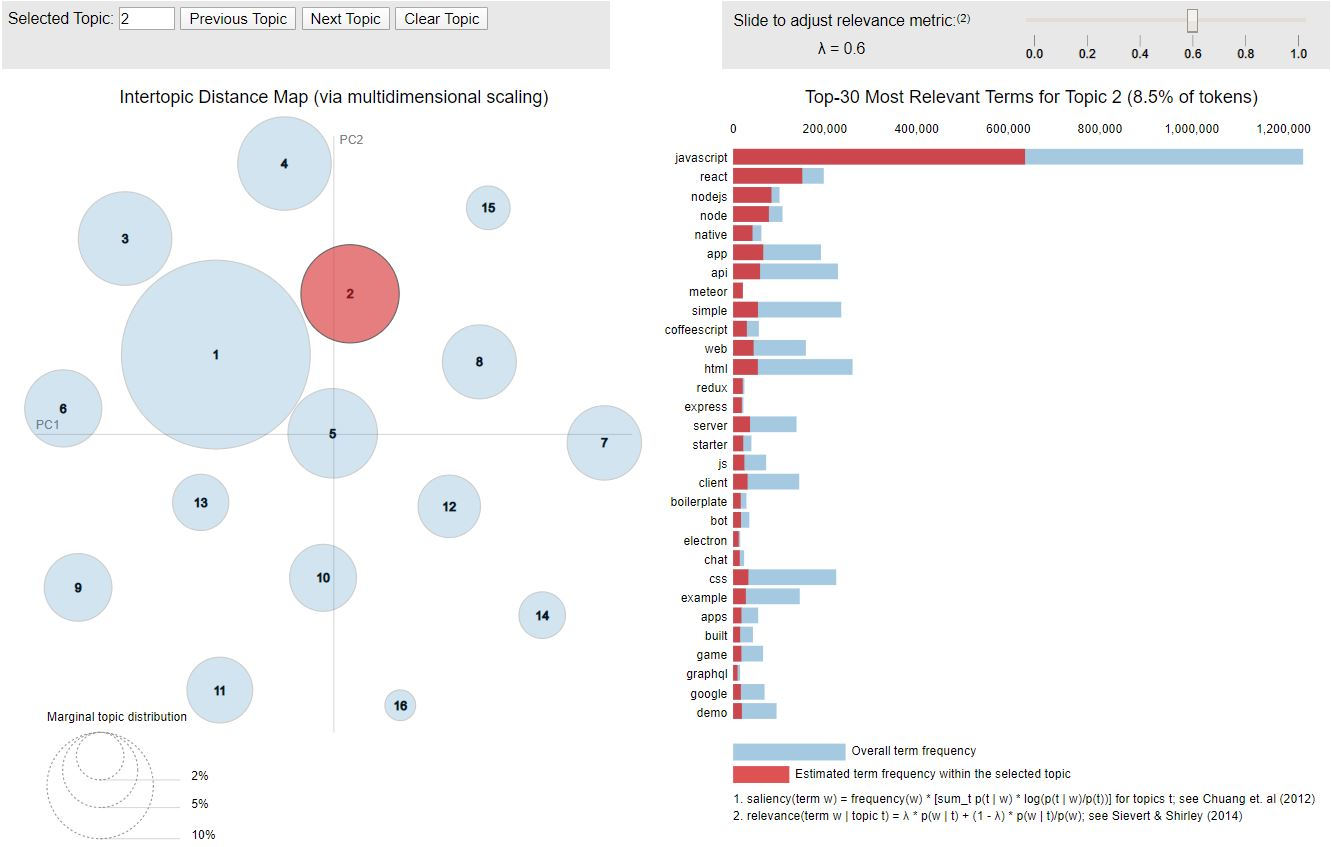
\includegraphics[width=\textwidth]{figures/pyLDAviz_GH.JPG}\\
              \caption{Visualization of the best LDA model fitted on GitHub data}
              \label{fig:pyldaviz_GH}
            \end{figure}
            
            \begin{figure}
              % Requires 
              \centering
              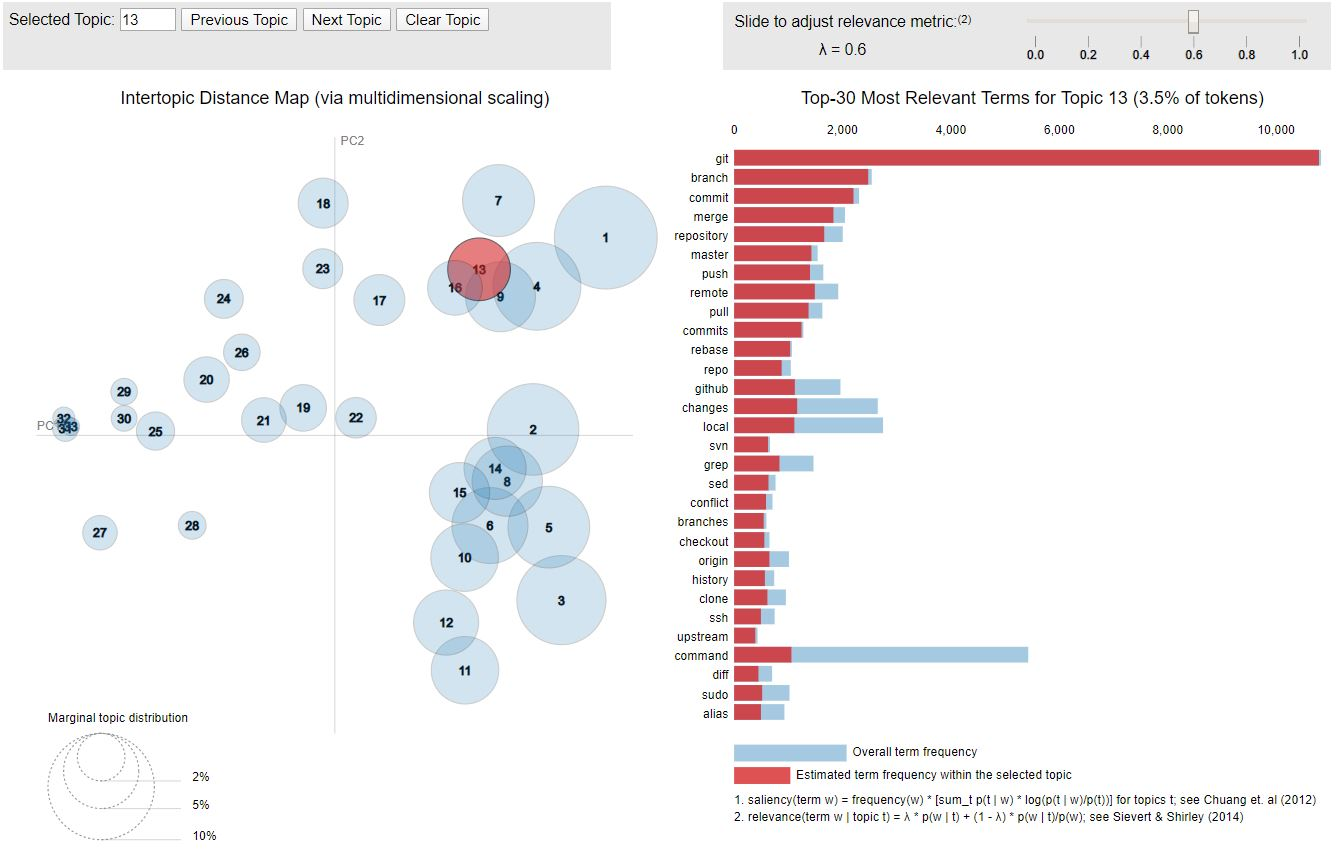
\includegraphics[width=\textwidth]{figures/pyLDAviz_SO.JPG}\\
              \caption{Visualization of the best LDA model fitted on Stack Overflow data}
              \label{fig:pyldaviz_SO}
            \end{figure}
    
    
    
    
    
    
    
    
    
    
    
    
